\documentclass[12pt,a4paper]{article}
\usepackage {amsmath,amsthm}
\usepackage{geometry}
\usepackage{titlesec}
 \geometry{a4paper, total={170mm,257mm}, left=20mm, right=20mm, top=25mm, bottom=25mm}
\usepackage{sectsty}
\usepackage{natbib}
\usepackage[hidelinks]{hyperref}
\usepackage{multirow}
\usepackage{makecell}
\usepackage{adjustbox}
%\usepackage{ulem}
\usepackage{threeparttable}
\usepackage{soul}
\usepackage[title]{appendix}
%\usepackage{prettyref}

%\usepackage[colorlinks=true, urlcolor=Blue]{hyperref}
%\usepackage{titling}
\sectionfont{\fontsize{14}{15}\selectfont}
\subsectionfont{\fontsize{13}{15}\selectfont}

\titleformat*{\section}{\LARGE\bfseries}
\titleformat*{\subsection}{\Large\bfseries}


\usepackage{caption}
\captionsetup{belowskip=0pt,aboveskip=6pt}

\makeatletter
\setlength{\@fptop}{0pt}
\makeatother

\makeatletter
\newcommand*\exInput[1]{\@@input#1 }
\makeatother


\usepackage[dvipsnames]{xcolor}
\newcommand{\fnote}[1]{\captionsetup{font={small, it}, aboveskip=0pt} \caption*{#1}}
\newcommand{\link}[1]{{\color{blue}\href{#1}{#1}}}

%TRACKING TOOL FOR ARYA: 
\newcommand{\agt}[1]{{\color{OliveGreen}#1}}
\newcommand{\agbf}[1]{{\noindent\textcolor{red}{TO DO:} \color{orange}\textbf{#1}}}
\newcommand{\agst}[1]{{\color{OliveGreen}\st{#1}}}

%TRACKING TOOL FOR ALEX: 
\newcommand{\aut}[1]{{\color{Red}#1}}
\newcommand{\aust}[1]{{\color{Red}\st{#1}}}

%TRACKING TOOL FOR Peter: 
\newcommand{\pmt}[1]{{\color{Blue}#1}}
\newcommand{\pmst}[1]{{\color{Blue}\st{#1}}}


%\usepackage{cite}
\usepackage{booktabs}
\usepackage{float}
\usepackage{setspace}
\usepackage{placeins}
\usepackage[list=true]{subcaption}
\captionsetup[sub]{font=footnotesize}

\usepackage{graphicx}


\newtheorem{theorem}{Proposition}
\newtheorem{hypothesis}{Hypothesis}
	\def\hypothesisautorefname{Hypothesis}
\newtheorem{result}{Result}
	\def\resultautorefname{Result}
\def\sym#1{\ifmmode^{#1}\else\(^{#1}\)\fi}


%\title{\Large Willingness to Pay for Signals of Rare Events\\}
\title{\Large Preferences for Warning Signal Quality: Experimental Evidence\\}

\author{Alexander Ugarov\thanks{Email: \href{mailto:augarov@hivereview.org}{augarov@hivereview.org}.} \\
{\small \textit{Hivereview}}
\and Arya Gaduh\thanks{Email: \href{mailto:agaduh@walton.uark.edu}{agaduh@walton.uark.edu}.} \\
{\small \textit{University of Arkansas}}\\
{\small \textit{and NBER}} 
\and Peter McGee\thanks{Email: \href{mailto:pmcgee@walton.uark.edu}{pmcgee@walton.uark.edu}.} \\
{\small \textit{University of Arkansas}} 
}

\begin{document}
\maketitle
\onehalfspacing
\begin{abstract}{
\noindent We use a laboratory experiment to study preferences over false-positive and false-negative rates of warning signals for an adverse event with a known prior. We find that subjects decrease their demand with signal quality, but less than predicted by our theory. They disproportionately reduce their demand for signals with high false-negative rates for rare events, while the opposite holds true for frequent events. We show that neither risk preference nor Bayesian updating skills can fully explain our results. Our results are most consistent with a decision-making heuristic in which subjects do not distinguish between false-positive and false-negative errors. 
%We conduct a laboratory experiment to study preferences over false-positive and false-negative rates of warning signals for an adverse event with a known prior probability. We find that subjects decrease their willingness-to-pay with signal quality, but less than predicted by our theory. They also disproportionately reduce their willingness-to-pay for signals with high false-negative rates for rare events, while the opposite holds true for frequent events. We explore potential channels and show that neither risk preference nor Bayesian updating skills can fully explain our results, which are most consistent with a decision-making heuristic in which subjects do not distinguish between false-positive and false-negative errors. 

%Information is often sought and used to protect against adverse events. We conduct a laboratory experiment to evaluate preferences over false-positive and false-negative rates of warnings signals and find significant deviations from the predictions of the model with a risk-neutral decision-maker as well as from some predictions of expected utility framework in general. Relative to a risk neutral decision-maker, willingness-to-pay overreacts to false-negative (FN) rates for low priors, and underreacts to FN rates for high priors, while subjects' preferences demonstrate a reverse bias for false-positive (FP) rates. As a consequence, subjects overpay for signals with positive FP rates when the prior is low and for all priors for signals with both positive FP and FN rates, i.e., low-quality signals. We find that the observed choices are most consistent with a decision-making heuristic in which subjects do not differentiate between false-positive and false-negative rates when choosing signals.
}


\vspace{10pt}
\begin{singlespace}
\noindent {\footnotesize{}JEL Classification: C91, D81, D84, D91}{\footnotesize \par}

\noindent {\footnotesize{}Keywords: alarms, value of information, information economics, information design, medical tests}{\thispagestyle{empty}}
\end{singlespace}
\end{abstract}

\vspace{180pt}
\newpage
\normalsize

\section{Introduction}

The trade-offs between false-positive and false-negative errors of warning systems often have life-and-death consequences. The 2010 gas blowout on the Deepwater Horizon oil rig killed 11 workers and caused one of the largest oil spills in history. The death toll was possibly aggravated by switching off the general safety alarm because the rig ``did not want people woke up at 3 a.m. from false alarms'' \citep{brown_oil_2010}. In medicine, different expert groups often disagree with the cancer screening guidelines issued by the U.S. Preventive Services Task Force, in large part over their perceived trade-offs between the costs from missed early detection against the potential harms from overdiagnosis or overtreatment due to false positive results \citep{rabin_reversal_2024}.

Most real-world warning systems --- medical diagnostics, security alarms, extreme weather alerts --- transform continuous signals about the likelihood of an adverse state into a yes/no binary signal. This transformation requires choosing a threshold for a positive classification. A lower threshold lowers the probability of failing to warn of an adverse state (false-negative rate) but increases the probability of warning in a safe state (false-positive rate), reflecting the standard trade-off characterized in ROC analysis \citep{fawcett_introduction_2006}. While the optimal threshold depends on user preference over the costs of these probabilistic errors, currently there is no guidance on what this threshold might be beyond assuming that decision-makers weigh false-positive and false-negative costs equally.\footnote{We define false positive and false negative \textit{costs} formally in Section 2, but it is important to keep in mind how they differ from false positive and false negative \textit{rates}.  False positive (negative) costs are the expected monetary costs to the decision maker as a function of the false positive (negative) rates and prior probabilities.}


%Our laboratory experiment indeed finds that most potential users of a warning system would prefer facing higher false-positive costs compared to a rational risk-neutral decision maker. 
To address this gap, we conduct a laboratory experiment to measure the demand for warning signals with varying quality.
%The experiment examines both demand for warning signals with known qualities and their utilization in protection decisions. 
In the experiment, subjects receive information about the prior probability of an adverse event and are asked to take a protective action after receiving a signal with known false-positive and negative rates. We then elicit our main outcome, i.e., their willingness-to-pay (WTP) for each signal. To account for subject heterogeneity, we use separate experimental tasks to measure their risk preference and Bayesian updating skill.

We compare the behavior of our subjects to that of a risk-neutral, utility-maximizing decision maker that we derive from a simple model. Subjects' WTP is weakly correlated with the value of information, resulting in overpaying for low-quality signals and underpaying for high-quality signals. Importantly, we find asymmetric under-responsiveness by prior: 
%subjects overreact to false-negative (false-positive) rates when the prior is low (high). 
with a low (high) prior, their WTP does not fully adjust for the increase in the false-positive (false-negative) costs.
We provide evidence that this pattern is most consistent with a failure to estimate the effect of the frequencies of false-positive and false-negative outcomes on the potential costs of using the signal. 

We contribute to the literature in three ways. First, we provide novel evidence on the demand for warning systems using an incentivized experiment. Existing studies of warning systems, which mostly focus on medical diagnostic tests, use unincentivized surveys to measure WTP and do not explore preferences over the tests' information structures. They find that preferences over diagnostic tests correlate with their accuracy, but respondents exhibit two significant biases. First, they are willing to pay for tests with little or no diagnostic value \citep{schwartz_enthusiasm_2004, neumann_willingness--pay_2012}. For example, \citet{schwartz_enthusiasm_2004} find that 73\% of Americans prefer a free full-body CT scan versus \$1,000 in cash even though full-body scans for healthy people are not recommended by physicians. Second, the way the information about the test's accuracy is presented strongly affects choices \citep{howard_does_2009}. We extend this literature using a context-neutral experiment to examine whether similar biases hold more generally and when choices are incentivized, as well as whether the demand elasticity for information responds symmetrically to false positive and false negative errors. 

Second, we contribute to the emerging experimental literature on the demand for information by studying signals that affect protection decisions. Previous studies in this literature employ prediction games, in which subjects must guess an optimal state under uncertainty \citep{hoffman_how_2016, ambuehl_belief_2018, xu_revealed_2022, MontanariNunnari2023}. Generally, they find that while the demand for information increases with signal quality, it increases more modestly than expected from a Bayesian decision maker. Two of these studies employ laboratory experiments. \citet{ambuehl_belief_2018} find that subjects underreact to the accuracy of a binary signal about the state of the world, but put a premium on completely certain signals. \citet{xu_revealed_2022} shows that many subjects choose non-instrumental signals over instrumental signals, consistent with failures in contingent reasoning about the future value of information and with partial failures to distinguish FP and FN rates. Both studies employ a prediction game.

% Our setup differs from those of \citet{ambuehl_belief_2018} and \citet{xu_revealed_2022}. 
We extend this literature by moving beyond a prediction game and instead incorporating protection decisions with three distinct payoffs (i.e., full payoff, full payoff minus protection costs, and full payoff minus losses). With asymmetric payoffs, risk preferences affect the value of information and can change sensitivities to false-positive and false-negative rates. Asymmetric payoffs also creates asymmetry in how subjects value different types of errors which is not observed in (symmetric) prediction games. We also directly elicit both willingness-to-pay and potential protection decisions for different combinations of priors and signal characteristics, allowing for more general conclusions about subjects' preferences. Consistent with \citet{ambuehl_belief_2018}, our subjects overvalue inaccurate signals, but we do not find a premium for signals with high certainty.  

Additionally, the subject's choices after receiving a signal in our experiment are equivalent to insurance decisions with full coverage. Hence our results also apply to insurance problems when subjects receive additional signals of their risks (such as flood zone designations). While on average people under-insure with respect to rare natural disasters \citep{friedl_insurance_2014}, the demand for insurance goes up immediately after an insurable adverse event \citep[e.g.,][]{kousky_understanding_2011}. One suggested explanation is that subjects overweight recent evidence leading to under-insurance when there were no negative events in the recent past and to overinsurance after the fact \citep{volkman-wise_representativeness_2015}. This is consistent with underweighting prior probabilities relative to more recent signals. At the same time, however, \citet{laury_insurance_2009} find no under-insurance for low-probability events in the laboratory setting.  We similarly find that, on average, subjects do not under-insure after receiving a signal even though we see potential over-protection for negative signals.

The paper proceeds as follows. The next section sets up a simple model and outlines our hypotheses. Section~\ref{sec:design} describes the experimental design. Given the novelty of some of the experimental tasks, we present our results in three consecutive sections. First, we describe a theory-free exposition of subjects' choices in all treatments in Section~\ref{sec:sanity}. Then, Section~\ref{sec:results} describes the results for main empirical tests of this paper with regards to the willingness-to-pay for signals. Finally, we explore potential explanations for the observed pattern of underreaction to false-positive rates for low initial probabilities in Section~\ref{sec:discussion}. Section~\ref{sec:conclusion} concludes. 


\vspace{20pt}
\section{Model}\label{sec:model}
\paragraph{Environment.} Let $\omega \in \{0,1\}$ denote the state of the world, where 1 corresponds to an adverse event that happens with probability $\pi$ and induces a loss, $L$. An agent can take protective action $a\in\{0,1\}$ to avoid losing $L$ under the adverse state. The loss is realized only when $\omega(1-a)=1$.

The agent's preferences are described by a utility function that depends on wealth $Y$, protective action $a$, and the protective outcome $\omega(1-a)$. Taking the protective action costs $c>0$ as given, utility is separable in wealth, protection cost, and the potential loss $L>c$ in the adverse state if not protected:
\[
U=U(Y,a,\omega(1-a))=u(Y-ac-\omega(1-a)L)
\]

The agent can purchase information in the form of a binary signal $s\in\{0,1\}$ about the state of the world. Let $P_{ij}\equiv P(s=i|\omega=j)$ be the probability that signal $s$ takes the value $i$ conditional on the state of the world being $j$.  After learning the signal's value, the agent updates her belief on the likelihood of the adverse event to $\mu(s)$. We assume that she is Bayesian and her posterior belief equals to:
\[
\mu(s)= {\pi P_{s1} \over \pi P_{s1}+(1-\pi)P_{s0}}
\]
where a larger $\mu(s)$ implies a higher posterior probability of the adverse event.

Without loss of generality, we assume information structure in which a positive signal $s=1$ is more likely in the adverse state of the world $P_{11}>P_{10}$.

\vspace{10pt}
\paragraph{Strategy.} Without a signal, the agent can choose only between always protecting and never protecting resulting in the following expected utility:
\[
U_0=\max[u(Y-c),\pi u(Y-L)+(1-\pi) u(Y)]
\]
With a signal, the subject's  strategy $\sigma:\{0,1\}\to\{0,1\}$ describes protection action for each signal's value.  We can represent it as a tuple of numbers $(a_0,a_1)$. Let $b\geq 0$ be the price of a signal paid beforehand from initial wealth and use $U(\sigma, b)$ to describe expected utility with a signal conditional on strategy and information price. Note that if the strategy is not responsive to the signal, payoffs cannot improve upon payoffs available without a signal because for any \(b>0\)\\
\[U(\sigma=(0,0),b)=\pi u(Y-L-b)+(1-\pi) u(Y-b)<\pi u(Y-L)+(1-\pi) u(Y)\]
i.e., choosing not to protect irrespective of the signal makes one worse off than just not purchasing the signal, and
\[U(\sigma=(1,1),b)=u(Y-c-b) <u(Y-c) \]
i.e., choosing to always protect irrespective of the signal makes one worse off than just not purchasing a signal.  If a subject follows the signal her expected utility is:
\[
U(\sigma=(0,1),b)=\pi P_{11}u(Y-c-b)+\pi P_{01}u(Y-L-b)+(1-\pi)P_{10}u(Y-c-b)+(1-\pi)P_{00}u(Y-b)
\]

Given our assumption that $P_{11}>P_{10}$, the expected utility of following the signal is higher than the expected utility of following the ``do the opposite" strategy:
 \[
U[\sigma=(1,0),b]=\pi P_{01}u(Y-c-b)+\pi P_{11}u(Y-L-b)+(1-\pi)P_{00}u(Y-c-b)+(1-\pi)P_{10}u(Y-b)
\]

Hence, value of the signal, i.e., the maximum willingness to pay for it, is determined by comparing the expected utility of following the signal (the LHS of eqn. 1) with the expected utility of not using a signal (the RHS of eqn. 1):
\begin{equation}
\max_\sigma U(\sigma,b)=U_0=\max[u(Y-c),\pi u(Y-L)+(1-\pi) u(Y)]
\end{equation}

As noted above, the signal's value cannot be positive if it is not followed, hence it should satisfy:
\begin{equation}\label{eq:devVal}
\begin{split}
P(s=1)u(Y-b-c)+\pi P_{01}u(Y-b-L)+(1-\pi)P_{00}u(Y-b)=\\=\max[u(Y-c),\pi u(Y-L)+(1-\pi) u(Y)] 
\end{split}
\end{equation}
where $P(s=1)\equiv \pi P_{11}+(1-\pi)P_{10}$. The expression on the left-hand side of this equation is a strictly decreasing function of $b$. Additionally, for $b\rightarrow \infty$ the left-hand side is smaller than the right-hand side. It implies that equation~(\ref{eq:devVal}) has at most one positive solution.

Obviously, $b>0$ for a perfectly accurate signal because the payoff distribution with the signal first-order stochastically dominates the distribution without it. However, determining the value of an imperfect signal is non-trivial, as it requires more restrictions on preferences to allow weighing outcomes with losses vs outcomes with protection costs.


\paragraph{Risk-neutral agent.} If the agent is risk-neutral, the expression above collapses to:
\[b+P(s=1)c+\pi P_{01}L=\min[c,\pi L]
\]
The signal's value is just:
\[
b^*=\max[0,\min[c,\pi L]-P(s=1)c-\pi P_{01}L]
\]

We can express the WTP for the signal, $b$, as a function of priors, false-positive (FP), and false-negative (FN) \textit{rates}  denoted correspondingly as $P_{10}$ and $P_{01}$. The following equation serves as our benchmark in the empirical work:
\begin{equation}\label{eq:rnWTP}
b=\max[0,\min[c,\pi L]-\pi (1-P_{01})c-(1-\pi)P_{10}c-\pi P_{01}L]
\end{equation}
The signal's value is decreasing in both FP and FN rates. The effect is proportional to the non-adverse (adverse) state probability for the FP (FN) rate. When WTP is positive ($b>0$),  its derivatives with respect to FP ($P_{10}$) and FN ($P_{01}$) rates are given by:
\begin{equation}\label{eq:dWTP_dFP}
{db\over dP_{10}}=-(1-\pi)c
\end{equation}

\begin{equation}\label{eq:dWTP_dFN}
{db\over dP_{01}}=-\pi(L-c)
\end{equation}
\vspace{10pt}

Note also that WTP is always equally affected by FP and FN \textit{costs} which are defined as $\pi (1-P_{01})c$ and $\pi P_{01}L$, respectively.

\paragraph{Risk Preferences.} In an expected utility framework, risk aversion can either increase or decrease an agent's valuation of the signal. More specifically, risk aversion decreases her WTP when protection costs are low: 

\begin{theorem}
 If the probability of the adverse state is high (i.e., $\pi>c/L$), then a strictly risk-averse decision-maker pays less than a risk-neutral one.
\end{theorem} 
\begin{proof}
See the Appendix.
\end{proof}

Intuitively, risk-averse decision-makers protect by default without using a signal when protection costs are sufficiently low. Things are less clear with low risks or higher protection costs. For example, if a risk-averse decision-maker chooses to not protect without a signal, risk aversion increases the value of a perfect signal. This follows from the standard argument that demand for insurance increases with risk aversion, and the fact that the protection problem with a perfect signal is isomorphic to the insurance problem with deductible $c$. 

Next, we examine the effect of the false-positive and false-negative rates of a signal on WTP, $b$. Assuming a differentiable utility function $u(.)$, we use implicit differentiation to derive sensitivities of $b$ to false-positive (FP) and false-negative (FN) rates:

\begin{equation}
\label{eq:senFP}
	{db\over dP_{10}}=-{(1-\pi)(u(Y-b)-u(Y-c-b))\over D(\pi, P_{01}, P_{10}, b)}
\end{equation}
\begin{equation}
\label{eq:senFN}
	{db\over dP_{01}}=-{\pi(u(Y-c-b)-u(Y-L-b))\over D(\pi, P_{01}, P_{10}, b)}
\end{equation}
with the denominator equal to the expected marginal utility:
$$D(\pi, P_{01}, P_{10}, b)\equiv P(S=1)u'(Y-c-b)+\pi P_{01}u'(Y-L-b)+$$
$$+(1-\pi)P_{00}u'(Y-b)=E[MU]>0$$
The signal's value decreases in FP and FN rates, i.e., ${db\over dP_{10}}$ and ${db\over dP_{01}}<0$. 
Equations~\ref{eq:senFP}-s~\ref{eq:senFN} indicate that risk aversion can either increase or decrease the decision-maker's sensitivity to FP and FN rates depending on the utility function's curvature and the signal's characteristics. Intuitively, the expected marginal utility of a strongly risk-averse subject with an imperfect signal can be lower than the average slope of the utility function between ($Y-c-b$) and ($Y-b$) which reduces sensitivity to FP rates. It can also be higher if either the signal is perfect or the curvature is small. Similarly, sensitivity to FN rates also depends on the form of the utility function.

However, we can say more about the ratio of sensitivities to FP and FN rates. For information structures in which both risk-averse and risk-neutral subjects purchase a signal, the ratio of sensitivities to FP rates over FN rates should be lower for strictly risk-averse subjects. 

\begin{theorem}
Conditional on both risk-neutral and risk-averse subjects purchasing a signal, strictly risk averse subjects have lower relative sensitivity to FP rates as compared to risk-neutral ones.
\end{theorem}\label{thm:riskAverse2}  

\begin{proof}
See the Appendix.
\end{proof}



\begin{center} * * * \end{center}
The model offers two testable hypotheses on the WTP that can be brought to the experiment. \emph{First,} as a natural starting point, we can test whether subjects' WTPs are equal to the values predicted for risk-neutral expected-utility maximizers given in equation 2. \emph{Second,} the model of a risk-neutral agent suggests that subjects' WTP should have equal sensitivity to \emph{costs} from false-positive and false-negative signals (equation~\ref{eq:rnWTP}). 

\section{Experimental Design}\label{sec:design}

We conducted the experiment using Qualtrics in the Behavioral Business Research Lab (BBRL) at the University of Arkansas. We conducted two waves of data collection with a total of 207 subjects. The first wave was conducted between October and November 2021 with 105 subjects, while the second wave was conducted between October and November 2025 with 102 subjects.  On average, including a \$5 show-up fee, subjects earned \$25.50 for a session lasting around 45 minutes. 
 
Subjects were endowed with \$25 (on top of the show-up fee) that they could potentially lose in the experiment. Their payoff was determined by their decisions in four sets of tasks played in the following order: (i) Blind Protection; (ii) Informed Protection; (iii) Belief Elicitation; and (iv) Willingness-to-Pay Elicitation. Subjects took a quiz of understanding prior to each task; the correct answer and an explanation were provided if a subject answered a question incorrectly.\footnote{Incorrect quiz answers for the Informed Protection section resulted in subjects facing three additional multiple choice questions. We believe that a clear understanding of the Informed Protection task is essential for subsequent tasks, hence the additional questions. Complete details of the comprehension questions are in the appendix.} Each task consisted of 6 rounds, resulting in 24 total rounds. At the end of the experiment, one of these 24 rounds is randomly selected as the payment round. The instructions can be found in the appendix.


\bigskip
\noindent\textbf{Blind Protection (BP)}\ \ \ Subjects decide whether to pay \$5 to protect against an adverse event: a random draw of a black ball.  Subjects know the prior probability that a black ball is drawn. A subject who draws a black ball will lose nothing if they chose to protect and \$20 if they did not. The prior probability of drawing a black ball across the 6 rounds is denoted as $p \in \{0.05,0.10,...,0.3\}$. The order was common for all the subjects, increasing monotonically from the lowest probability. Subjects did not receive feedback on the decision's outcome.

\bigskip
\noindent\textbf{Informed Protection (IP)}\ \ \ As in the BP task, subjects must make a protection decision before learning if they drew a black ball. Prior to the protection choice, subjects learn the prior probability of drawing a black ball, receive a signal about the ball, and learn the signal's information structure. Following \citet{coutts_good_2019}, we represent this information structure using a group of hinting gremlins, where the hint is provided by a randomly selected gremlin (mapping to a signal realization in the model). The gremlin is one of three types: (i) honest; (ii) ''black-swamp'' who always says that the ball is black; and (iii) ''white-swamp'' who always says that the ball is white. Figure~\ref{fig:Gremlins} illustrates how these gremlin types were presented to the subjects. The group composition determines the information structure: a higher share of black(white)-swamp gremlins produces a signal with higher FP (FN) rate. Subjects know the group composition, but do not know which gremlin provides the signal in any particular round. Subjects are asked to make two protection decisions, to wit, for black and white signals.

\begin{figure}[H]
\centering
\caption{Signals Presentation} \label{fig:Gremlins}
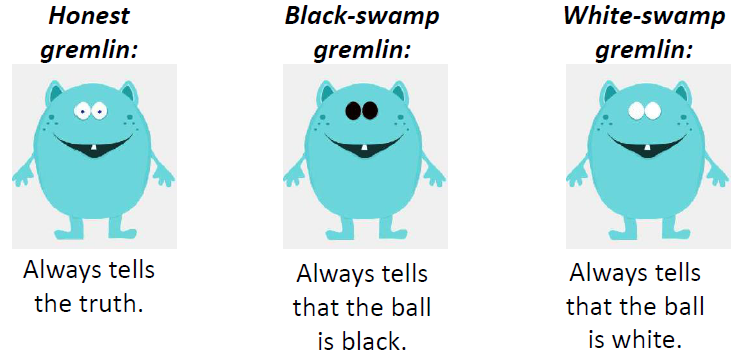
\includegraphics[width=0.6\textwidth]{Graphs/gremlins1.png}
\end{figure}
%\footnote{\agt{XXX If we want, we can discuss in this footnote that the term "honest" likely describes how people perceive the signal in real life, assuming we can find good anecdotes or studies XXX} \pmt{I couldn't find anything where they said people's perception of the test is "dishonest," but I did find things where people lose trust in tests and the people interpreting tests (i.e., doctors).  Unless someone else finds something particularly compelling, I'm not sure this is the way to go.  In the letter, we might be able to push back on it a bit because our elicitation is arguably less heavy-handed than Coutts' original.}}

\bigskip
\paragraph{Belief Elicitation (BE).} 
As in the IP task, subjects know the prior probability of drawing a black ball and the information structure (represented by the composition of the group of gremlins). Instead of making a protection decision, however, subjects are asked to estimate the probability that: (i) the ball is black when the gremlin says that it is white; (ii) the ball is black when the gremlin says that it is black.

To elicit incentive-compatible responses, we follow the stochastic version of the Becker-DeGroot-Marshak mechanism developed by \citet{grether_testing_1992} and \citet{holt_update_2009} but stated equivalently in terms of losses rather than gains.  Subjects submit their beliefs about the probability of the adverse event $\mu \in [0,1]$. If $\mu$ is above some uniform random number $r\in[0,1]$, they lose \$20 only if this event happens (i.e., a black ball is drawn). If $r > \mu$, then they draw an independent lottery that will lose \$20 with probability $r$ and 0 otherwise.\footnote{The benefit of this mechanism versus other probability elicitation mechanisms (e.g., quadratic scoring) is that reporting truthfully is a dominant strategy regardless of risk preferences \citep{karni_mechanism_2009-1} as long as a subject's preferences adhere to probabilistic sophistication and dominance i.e., they rank lotteries based on their probabilities only and prefer higher probabilities of higher payoffs.} \citet{danz_belief_2020} find that providing a detailed explanation of payoffs in belief elicitation lowers truthful reporting. Accordingly, our instructions begin by pointing out that reporting one's true belief $\mu$ maximizes payoffs, followed by an explanation of payoff calculation under different reporting strategies.

\paragraph{Willingness-to-Pay Elicitation (WTPE).} The WTPE task measures a subject's willingness to pay (WTP) for a signal. As before, subjects know the prior probability of drawing a black ball and the information structure of a potential signal.  Unlike the IP task, subjects do not automatically receive a signal, instead they provide their WTP for a signal by choosing a value $\in (\$0,\$5)$ in \$0.50 increments. The elicitation is incentive compatible: if a WTPE round is selected as the payment round, a random price for the signal is drawn. If that price exceeds the subject's WTP, they will play a BP round, otherwise the subject pays their WTP and plays an IP round after receiving a signal with the given information structure.  

\paragraph{Post-Experiment Questionnaire and Payment.}  After the WTPE task, subjects in both waves answered a few demographic questions: gender, age, education level, and on taking any statistics or probability classes. Subjects in the second wave also answered questions about their GPA, and the seven-item extended Cognitive Reflection Test (CRT) to measure their cognitive skills \citep{toplak_assessing_2014}. The payment task and the payment round were then randomly chosen to calculate the subject's payoff.

\paragraph{Treatments and Treatment Assignment.} Table~\ref{tab:treatments} summarizes our treatments for tasks other than BP. The treatments combine four priors with 12 different information structures for a total of 48 treatments. These treatments allow for a distribution of posteriors (for black and white signals) that spans a wide range of interior values and allows for a wide range of theoretical WTP values (Appendix Figure~\ref{fig:Value_hist}).

Subjects were assigned to treatments in the following manner. Each subject was randomly assigned six treatments that combined a pair of priors of either (0.1, 0.3) or (0.2, 0.5) with three information structures. The presentation of the treatments were organized by prior, and the order of the priors --- i.e., whether the first was larger than the second --- was randomly assigned. For each prior, the first treatment was always the one with a fully truthful information structure. The order of priors and signals stays constant for each subject across tasks, but can vary between subjects.

% For tasks other than BP, subjects go through two different priors and three types of signals. The order is such that subjects go consecutively over all three signal types starting from the honest one for each prior. The order of priors and signals stays constant for each subject across tasks, but can vary between subjects. \agt{We randomize across subjects whether the first of the two priors was larger than the second.} Table~\ref{tab:treatments} summarizes our treatments.
%\pmt{I haven't done this in the table, but I think we should take out the numeric column headers in Table 1}
%%%%%%%%%%%%%%%%%%%%%%%%%%%%%%%%%%%%%%%%%%%%%%%%%%%%%%%%%%%%%%%%%%%%%%%%%%%%%%%%%%%%%%%%%%%%%%%%%%%%%%%%
\begin{table}[h!]
\centering
\caption{List of Treatments} \label{tab:treatments}
\begin{tabular}{l*{6}{c}}
\hline\hline
 & \multicolumn{3}{c} {Number of Gremlins} & & \\ \cmidrule{2-4}
\multirow{2}{*}{Prior ($p$)} & \multirow{2}{*}{Total} & Black- & White- & \multirow{2}{*}{FP rate} &  \multirow{2}{*}{FN rate}\\
                    & &Swamp& Swamp \\
                    & (1) & (2) & (3)  & (4)  & (5)\\
[1ex]                    
\hline
0.1, 0.2, 0.3, 0.5         &    2 & 0  &  0 & 0.00 & 0.00\\
0.1, 0.2, 0.3, 0.5         &    2 & 1  &  0 & 0.50 & 0.00  \\
0.1, 0.2, 0.3, 0.5         &    2 & 0  &  1 & 0.00 & 0.5.0  \\
0.1, 0.2, 0.3, 0.5         &    3 & 1  &  0 & 0.33 & 0.00  \\
0.1, 0.2, 0.3, 0.5          &    3 & 0  &  1 & 0.00 & 0.33 \\
0.1, 0.2, 0.3, 0.5           &    3 & 1  & 1 & 0.33 & 0.33\\
0.1, 0.2, 0.3, 0.5         &    5 & 1  & 0 & 0.20 & 0.00\\
0.1, 0.2, 0.3, 0.5         &    5 & 0  & 1 & 0.00 & 0.20    \\
0.1, 0.2, 0.3, 0.5         &    5 & 1 & 1  & 0.20 & 0.20  \\
0.1, 0.2, 0.3, 0.5         &    7 & 2  &  0 & 0.29 & 0.00  \\
0.1, 0.2, 0.3, 0.5         &   7 & 0  &  2 & 0.00 & 0.29  \\
0.1, 0.2, 0.3, 0.5         &   7 & 1  &  1 & 0.14 & 0.14  \\
\hline\hline
\end{tabular}


\end{table}

%%%%%%%%%%%%%%%%%%%%%%%%%%%%%%%%%%%%%%%%%%%%%%%%%%%%%%%%%%%%%%%%%%%%%%%%%%%%%%%%%%%%%%%%%%%%%%%%%%%%%%%%

 
\section{Subject Decisions By Task}\label{sec:sanity}

Decisions in the Blind Protection (BP), Informed Protection (IP), and Belief Elicitation (BE) tasks measure determinants of WTP in our model. Protection choices in the BP task reveal subjects' risk preferences with known probabilities. Choices in the IP task demonstrate how subjects use signals given their characteristics. Finally, the BE task provides insight into subjects' beliefs for given signals.  
% We briefly discuss patterns of subject decisions below. They suggest that subjects understand these tasks reasonably well.

Given the complexities of some of these tasks, this section illustrates the extent of subject comprehension using simple descriptive analyses. We find that subjects understand these tasks reasonably well. This section also provides a qualitative overview of how subjects tend to deviate from the theoretical predictions for each task. We provide a more formal regression analysis of how signal characteristics affect subjects' WTP later in Section~\ref{sec:results}.

\subsection{Blind Protection}

Figure~\ref{fig:ProtResponse} plots the likelihood of protecting against the posterior probability of drawing a black ball for the BP task, where the posterior is equivalent to the prior (the thick line), and in the IP task (the thin line). On aggregate in the BP task, subjects' likelihood of protecting increases in the probability of an adverse outcome: only 13\% subjects protect when the probability of a black ball is 10\% in contrast to 70\% protecting when the probability is 30\%.

At the individual level, BP responses indicate significant heterogeneity in risk preferences. For approximately 70\% of subjects (143/206), protection action increases monotonically in probability. The remaining 30\% make at least one switch from protecting to not protecting and back, which is inconsistent with EU maximization.\footnote{That is, subjects do not protect for some treatments with posterior probability $P$ while protecting for a posterior probability $P'<P$.  Inconsistency on risk preference measures is well known.  \citet{filippin_reconsideration_2016} found that 17.1\% of more than 6,300 subjects in 54 published papers made inconsistent switches on the \citet{holt_risk_2002} paired-lottery measure. Among our switchers, however, 76\% (48/63) skip only a single increment of the presented probability scale, suggesting an inattention error.}

%\footnote{For comparison, Holt and Laury (2002) for a similar instrument find that 28 of 212 subjects (13\%) switched back to a low-risk option with an increasing likelihood of high payoffs in a risky option at least once when decisions were presented in increasing order, which they are not here.}

Risk-neutral agents who maximize their expected utility should start protecting when the prior exceeds 0.25, i.e., at the ratio of the protection cost to the potential loss (\$5/\$20). Many of our subjects (61, or 29\%) start protecting at lower priors (0.05-0.15), indicating strict risk aversion.  A smaller group of subjects makes choices consistent with risk loving by protecting at a probability of 0.3 or never.\footnote{As a reference using a CRRA utility function, switching at the probability 0.1 corresponds to a coefficient of relative risk aversion $\theta=2$, switching at 0.2 corresponds to $\theta=0.57$, and switching at 0.3 corresponds to $\theta=-0.54$.} 


\subsection{Informed Protection}

Recall that, in the IP task, subjects not only know the prior but also receive a signal about the ball color. 
Figure~\ref{fig:ProtResponse} shows that protection actions are increasing in the posterior probability of an adverse event, though roughly 28\% of subjects break monotonicity in their protection responses with respect to posterior probabilities. This is approximately the percentage of non-monotonic responses in the BP task.  Breaking monotonicity here is not particularly surprising as subjects are not directly given their posterior probabilities and may estimate them incorrectly. At the individual level, we also find that the total number of times subjects protect in the BP task significantly correlates with their likelihood of protection in the IP task conditional on posteriors, but this explains only a very small part ($<$1\%) of variation in the IP decisions.\footnote{We use a linear probability model to estimate this relationship with controls for posterior probability, reported belief, and hint, and while the coefficient on the total number of protection choices is significant at the 1\% level, the $R^2$ only increases from 0.41 to 0.42.} 


%%%%%%%%%%%%%%%%%%%%%%%%%%%%%%%%%%%%%%%%%%%%%%%%%%%%%%%%%%%%%%%%%%%%%%%%%%%%%%%%%%%%%%%%%%%%%%%%%%%%%%%%%%%%%%%%%%%

\begin{figure}[H]
\centering
\caption{Average Protection Response} \label{fig:ProtResponse}
  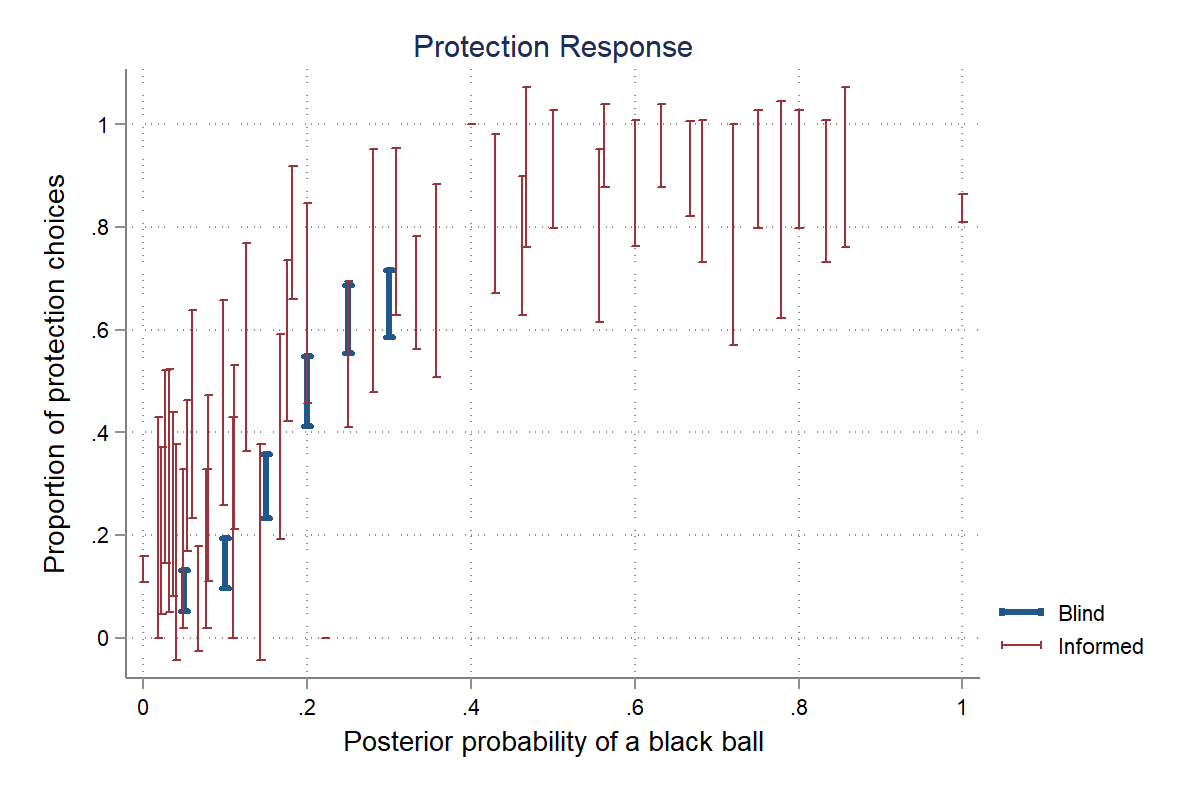
\includegraphics[width=0.7\textwidth]{Graphs/ip_response_comp.png}
\fnote{The bars show 95\% confidence intervals for the mean proportion of subjects choosing protection at each posterior probability.}
\end{figure}
%%%%%%%%%%%%%%%%%%%%%%%%%%%%%%%%%%%%%%%%%%%%%%%%%%%%%%%%%%%%%%%%%%%%%%%%%%%%%%%%%%%%%%%%%%%%%%%%%%%%%%%%%%%%%%%%%%%

Table~\ref{tab:nonparIP} presents the average protection decisions by prior and signal type. The first three columns indicate the signal and its information structure. Column 4 shows the posterior probability of a black ball averaged across all the treatments within a group. We calculate it from priors and FP and FN rates using the Bayes formula for each treatment and each signal value and then average across the subjects. Column 5 display the proportion of subjects who protect for corresponding treatment, and column 6 presents the weighted across treatments average of optimal responses for a risk-neutral decision maker. Finally, column 7 presents the $p$-value for a test of equality between empirical and theoretical protection responses.\footnote{In Appendix Table~\ref{tab:nonparIP_A}, we disaggregate the results by prior. The disaggregated results are largely similar to those in Table~\ref{tab:nonparIP}.}

Three observations emerge from the table. First, regardless of the signal's FP and FN rates, black signals substantially increase the likelihood of protection.  Second, subjects' protection decisions deviate significantly from what is optimal for risk-neutral subjects in most treatments, as evidenced by column 7. Subjects significantly overprotect when facing white signals (rows 1--4), while significantly underprotecting when facing black signals without false positives (rows 5--6). 

Third, we find deviations that cannot be explained by expected utility maximization for any degree of risk aversion. For example, consider rows 1 and 3: even though an increase in the FP rate does not change the posterior (because the signal is white), the protection rate increases by 23 percentage points. Similarly, comparing rows 3 and 4, we see that introducing FN rates to an information structure with an FP rate raises the protection rate increases to 41 percent --- even though the average posterior probability given the signal's characteristics is merely 8 percent. As a benchmark, with no signal in the BP task, only 15(30) percent of subjects choose to protect when the probability is 10~(15) percent. 

%%%%%%%%%%%%%%%%%%%%%%%%%%%%%%%%%%%%%%%%%%%%%%%%%%%%%%%%%%%%%%%%%%%%%%%%%%%%%%%%%%%%%%%%%%%%%

\begin{table}[H]\centering 
\caption{Average Protection by Signal Type} 
\label{tab:nonparIP}
\adjustbox{max width=\textwidth}{
	\begin{threeparttable}
	\begin{tabular}{cccccccc} \hline \hline
	\multirow{4}{6ex}{\centering \textbf{Row}}
            &\multirow{4}{12ex}{\centering \textbf{Signal}} 
			&\multicolumn{2}{c}{\centering \textbf{Signal Characteristics}} 
			& \multirow{4}{10ex}{\centering \textbf{Posterior}} 
            & \multirow{4}{10ex}{\centering \textbf{Share Protect}} 
			& \multirow{4}{10ex}{\centering \textbf{Share Optimal}} 
			& \multirow{4}{13ex}{\centering \textbf{$p$}} \\ %P-val $(H_0: (5)=(6))$
			\cmidrule(lr){3-4}
		      &
            & \multirow{2}{12ex}{\centering \textbf{False Positive}} 
			& \multirow{2}{12ex}{\centering \textbf{False Negative}} 
		\\
		\\
		&(1) & (2) & (3) & (4) & (5) & (6) & (7) \\
		\hline
			\input{Tables/bigpicture_IP_AU_cl.tex}
			\\[-1em]
		\hline\hline 
	\end{tabular} 
	\begin{tablenotes}[flushleft]
			\item\leavevmode\kern-\scriptspace\kern-\labelsep \footnotesize \textit{Notes:} The p-value in column 7 is for the test of equality between the theoretical prediction (column 6) and the observed share of protection (column 5). 
	\end{tablenotes}								
	\end{threeparttable}
	}
\end{table}



%\bigskip\noindent\textbf{Belief Elicitation.}\ \ \ 
\subsection{Belief Elicitation}
Subject decisions in the IP task capture the use of signals in protection decisions, but decisions reflect both risk preferences and (potentially erroneous) beliefs.  The BP task can be used to construct a measure of the former; the BE task measures the latter.  


%%%%%%%%%%%%%%%%%%%%%%%%%%%%%%%%%%%%%%%%%%%%%%%%%%%%%%%%%%%%%%%%%%%%%%%%%%%%%%%%%%%%%%%%%%%%%%%%%%%%%%%%%%%%%%%%%%%

\begin{figure}[H]
	\centering
	\caption{Errors in Bayesian Updating} \label{fig:BeliefUpdate}
	\subcaptionbox{Error Distribution}{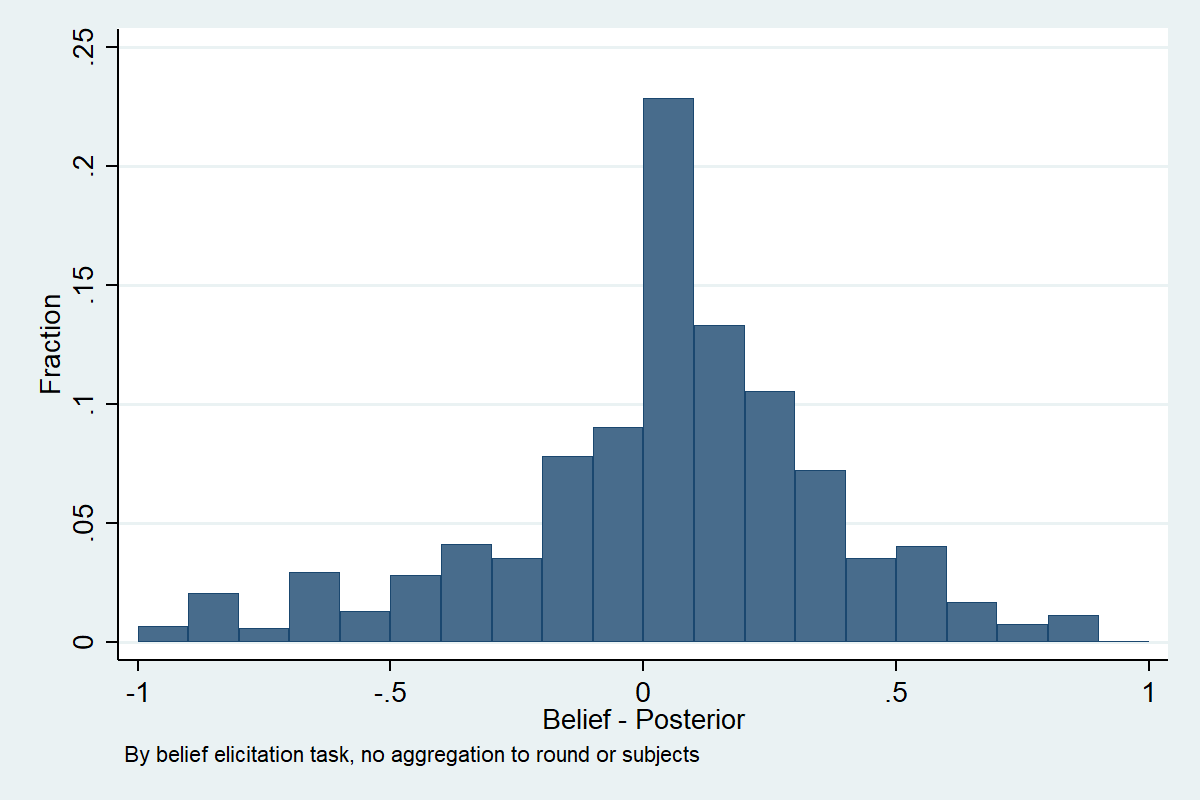
\includegraphics[width=.48\textwidth]{Graphs/hist_belief_errorw.png}}
	\hfill
	\subcaptionbox{Error v. Posterior}{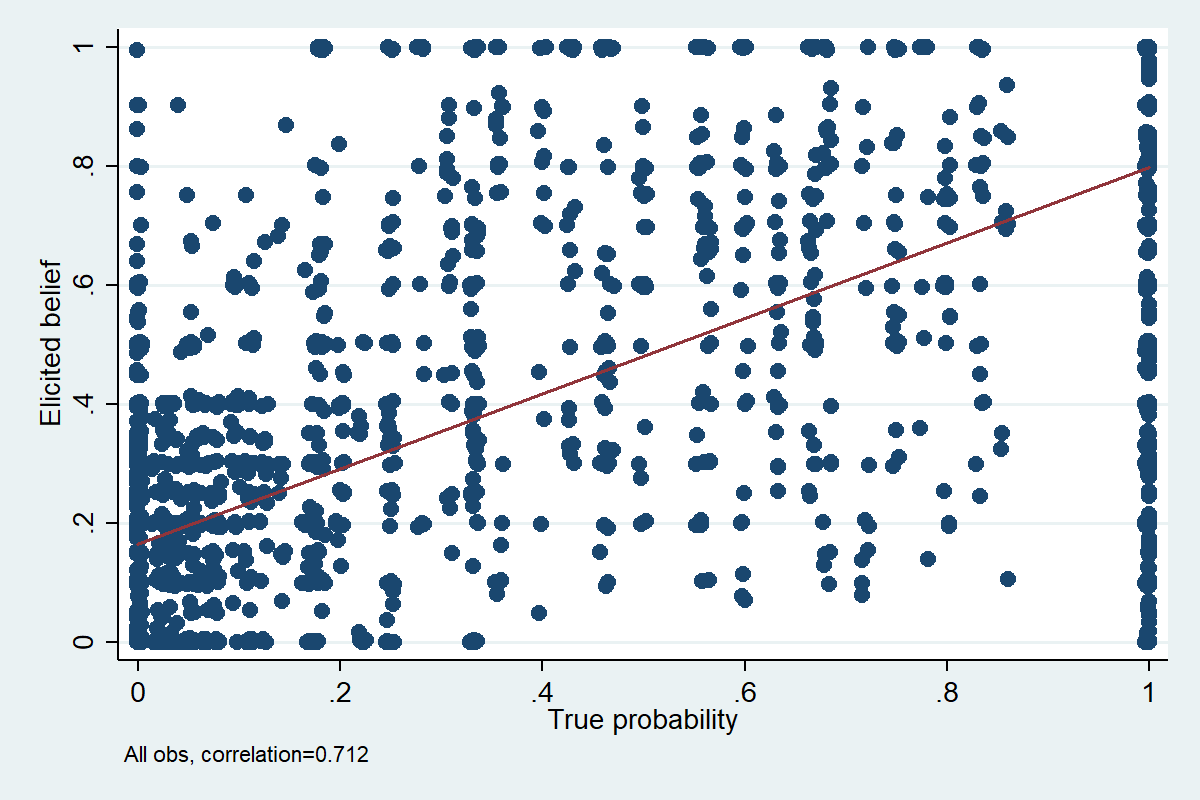
\includegraphics[width=.48\textwidth]{Graphs/updating_s1.png}}
	\hfill
	\vspace{2em}
	\subcaptionbox{Error Distribution, Certain Posterior}{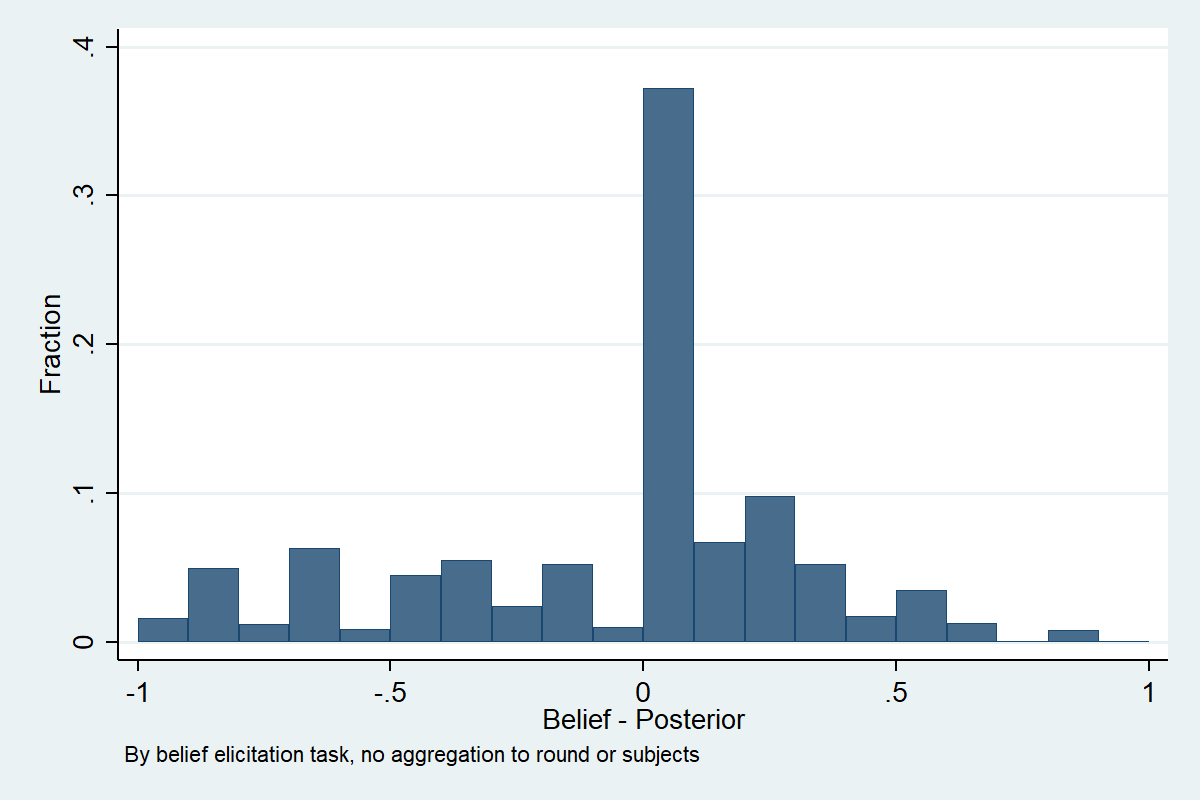
\includegraphics[width=.48\textwidth]{Graphs/hist_belief_error_s5w.png}}
	\hfill
	\subcaptionbox{Error v. Posterior, Certain Posterior}{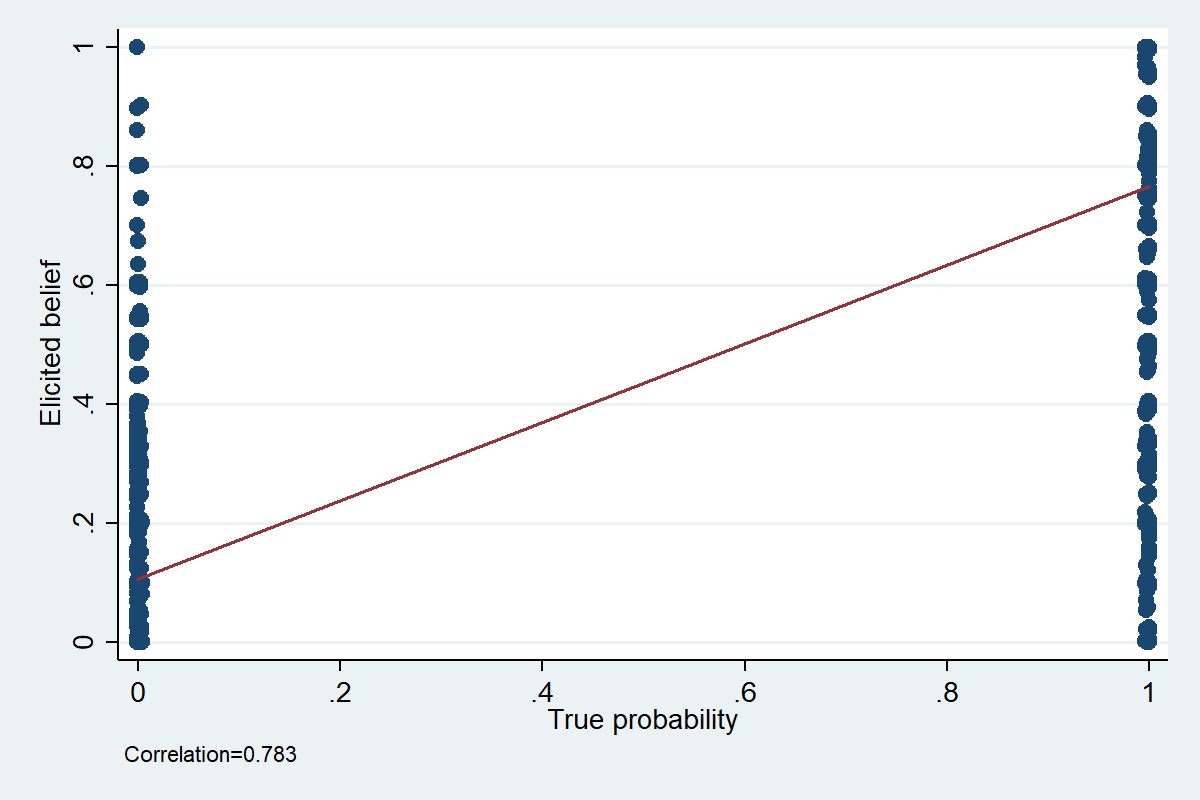
\includegraphics[width=.48\textwidth]{Graphs/updating_s5.png}}
	\hfill
	\vspace{2em}
	\subcaptionbox{Error Distribution, Uncertain Posterior}{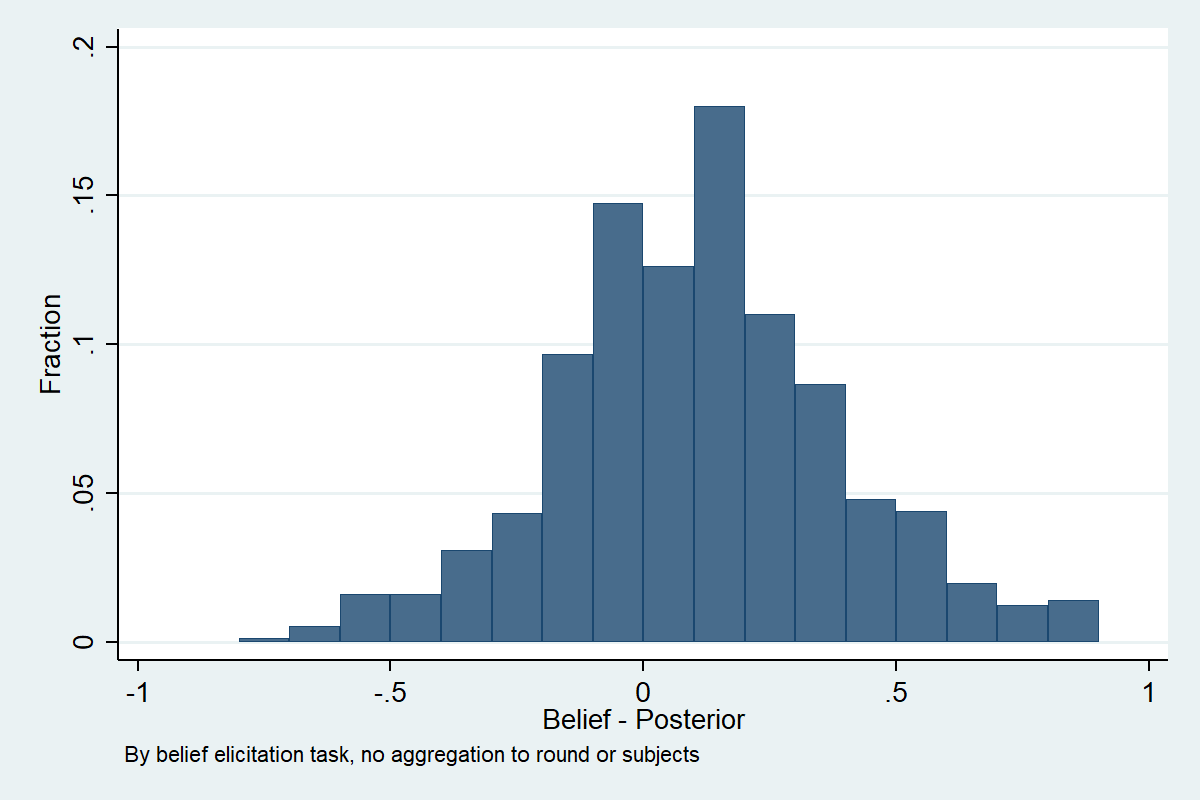
\includegraphics[width=.48\textwidth]{Graphs/hist_belief_error_s4w.png}}
	\hfill
	\subcaptionbox{Error v. Posterior, Uncertain Posterior}{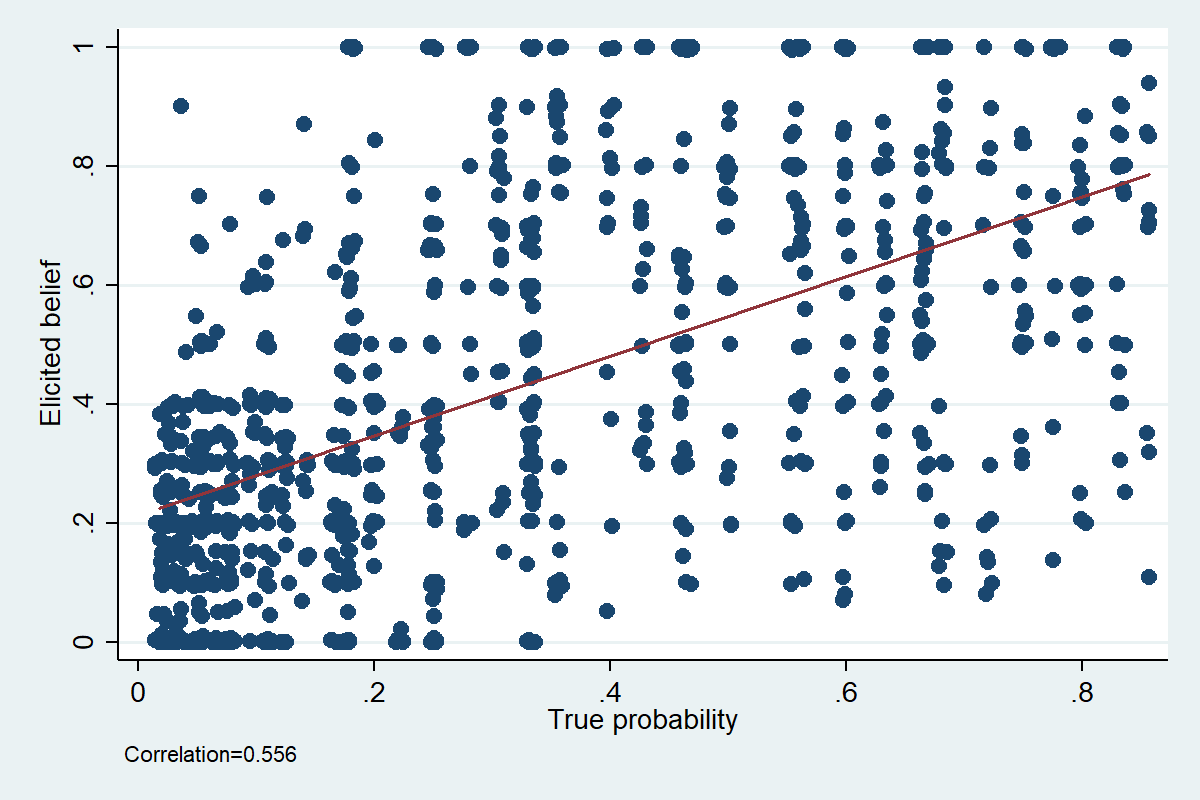
\includegraphics[width=.48\textwidth]{Graphs/updating_s4.png}}
	\hfill
    \makebox[0.9\textwidth][l]{%
        \parbox{0.9\textwidth}{%
            \footnotesize\textit{Notes:} The updating error is defined Belief - Posterior. Each observation is weighted by the inverse of its treatment frequency.
        }%
    }\end{figure}
%%%%%%%%%%%%%%%%%%%%%%%%%%%%%%%%%%%%%%%%%%%%%%%%%%%%%%%%%%%%%%%%%%%%%%%%%%%%%%%%%%%%%%%%%%%%%%%%%%%%%%%%%%%%%%%%%%%



We define updating errors as the difference between the subjects' elicited belief and the Bayesian posterior probability of drawing a black ball for a given signal. The left-hand column of Figure~\ref{fig:BeliefUpdate} shows the distribution of the updating errors, while its right-hand column presents a scatter plot of the elicited beliefs against the true posterior\footnote{Posteriors are calculated from priors and information structures using the Bayes formula.} with a fitted line. We re-weight the observations by the inverse its treatment frequency to ensure balance by treatment.\footnote{Since our treatment assignment was not balanced across treatments, we may give too much weight to information structures with certain characteristics absent this reweighting. For example, we would have put too much weight on treatments with a truthful information structure since there will always be a total of two treatments with (one for each prior) in every session.}

Panel A indicates that beliefs are still sensible despite errors. The distribution of updating errors is centered at 0, with roughly one-half (53\%) of errors concentrated within +/- 0.2 interval around zero. Overall, the correlation between the elicited beliefs and the true posteriors was 0.71 (Panel (b)).  

For some combinations of priors and signals, updating should be trivial and posteriors are completely certain.  
Panel~(c) plots such cases, which account for 57\% of the sample and include: (i) treatments with all-honest gremlins; and (ii) treatments with obviously irrelevant dishonest gremlins (e.g., a group comprising of only honest and white-swamp gremlins announcing that the ball is black --- or vice versa). Reassuringly, 78.3\% of reported beliefs in those cases are correct. About half of the errors involve reporting a probability of one when it should have been zero.

Meanwhile, Panel~(e) plots the remaining observations, i.e., those with uncertain posteriors. The median error in Panel~(e) is 0.11, with 90\% of errors lying between -0.36 and 0.57, suggesting that, on average, subjects overestimate the likelihood of adverse events for uncertain posteriors. The correlation between beliefs and posteriors in this sub-sample falls to 0.56.\footnote{The overall pattern of belief updating is consistent with the existing literature which shows that despite updating in the correct direction, people tend to underreact both to the priors and to the signals. The effect of underweighting priors --- first noted in the psychology literature \citep{phillips_conservatism_1966-1, tversky_belief_1971, kahneman_subjective_1972} --- is known as \emph{representativeness bias} or \emph{base-rate neglect}. Using the regression approach of \citet{grether_bayes_1980}, we find both base-rate neglect and signal underweighting. Our estimates of these parameters are significantly below one with $\hat \alpha=0.43$ $\hat \beta=0.25$ (see Column 1 in Appendix Table~\ref{belief_decomposition}). These values are within the range found by the meta-analysis of \citet{benjamin_chapter_2019} which calculates the average $\hat \alpha$ estimate to be around 0.22 (0.4 for incentivized studies only) and the average $\hat \beta$ to be 0.6 (0.43 for incentivized) for studies (like ours) that presented their signals simultaneously.  Such experiments are known as \emph{bookbag-and-poker-chip} experiments} 

%%%%%%%%%%%%%%%%%%%%%%%%%%%%%%%%%%%%%%%%%%%%%%%%%%%%%%%%%%%%%%%%%%%%%%%%%%%%%%%%%%%%%%%%%%%%%

\begin{table}[H]\centering 
\caption{Average Updating Error by Signal Type} 
\label{tab:nonparError}
\adjustbox{max width=\textwidth}{
	\begin{threeparttable}
	\begin{tabular}{ccccccc} 
	\hline \hline
		\multirow{4}{6ex}{\centering \textbf{Row}}

        
          &\multirow{4}{12ex}{\centering \textbf{Signal}} %P-val 
			&\multicolumn{2}{c}{\centering \textbf{Signal Characteristics}} 
            
			& \multirow{4}{10ex}{\centering \textbf{Posterior}} 
			& \multirow{4}{12ex}{\centering \textbf{Updating Error}} & \multirow{3}{12ex}{\centering \textbf{$p$}}  \\ \cmidrule(lr){3-4}
		& & \multirow{2}{10ex}{\centering \textbf{False Positive}} & \multirow{2}{12ex}{\centering \textbf{False Negative}} 
		\\
		\\
		& (1) & (2) & (3) & (4) & (5) & (6) \\
	
		\hline	
(1)&White&No&No&0.000&0.048&0.023\\
(2)&White&No&Yes&0.119&0.051&0.008\\
(3)&White&Yes&No&0.000&0.210&0.000\\
(4)&White&Yes&Yes&0.110&0.200&0.000\\
(5)&Black&No&No&1.000&-0.145&0.000\\
(6)&Black&No&Yes&1.000&-0.384&0.000\\
(7)&Black&Yes&No&0.512&0.161&0.007\\
(8)&Black&Yes&Yes&0.538&0.022&0.692\\

\\ 	[-1em]
\hline\hline
\end{tabular} 
	\begin{tablenotes}[flushleft]
			\item\leavevmode\kern-\scriptspace\kern-\labelsep \footnotesize \textit{Notes:} The updating error is defined as Belief - Posterior, where Posterior is the Bayesian probability estimate for the treatment based on its information structure. The p-value in column 6 is for the test of the null hypothesis that the updating error in column 5 is equal to 0.% $ \text{Updating error} = . 
	\end{tablenotes}								
	\end{threeparttable}
	}
\end{table}
%%%%%%%%%%%%%%%%%%%%%%%%%%%%%%%%%%%%%%%%%%%%%%%%%%%%%%%%%%%%%%%%%%%%%%%%%%%%%%%%%%%%%%%%%%%%%



Table~\ref{tab:nonparError} summarizes how updating errors vary with the information structure.\footnote{Appendix Table~\ref{tab:nonparError_A} disaggregates the results further by prior} We find that subjects overestimate the probability of a black ball when receiving a white signal, which is consistent with the overprotection in the IP task. This upward bias for a white signal increases in both the FP and FN rates of its information structure. To illustrate, consider the change between rows 1 and 3, where introducing an FP rate would not change the posterior (theoretical probability) because the signal is white. Yet, subjects update their beliefs upward, magnifying their updating error; we find a similar effect for the introduction of the FN rate (row 1 vs. 2).

The updating bias for black signals, however, varies by the information structure. Subjects slightly underestimate the probability with a perfectly accurate signal. However, a comparison of rows 5 and 6 suggests introducing FN rates to the information structure exacerbates subjects' underestimation. Black signals from an information structure with a non-zero FP rate leads to an overestimation of the probability of a black ball. Interestingly, adding a FN rate to the information structure attenuates this overestimation.

% The difference in the updating errors for black signals coming from FP-only (row 7) v. FP-FN signals (row 8) is negligible. 
% The magnitude of subjects' adjustments to their beliefs was smaller than the actual change to the posteriors due to the FP rates.

Subjects' choices in BE task are overall highly consistent with their choices in the IP task. We use the Mann-Whitney U-statistic to examine the number of cases when a subject inconsistently protects for a belief $\mu_1$ but does not protect for a belief $\mu_2\geq \mu_1$. The median U-statistic is 0.93, indicating an almost perfect rank correlation with just 1 or 2 discordant choices per subject; 35\% of subjects report beliefs which are fully consistent with their protection decisions. At the same time, there is a minority of subjects with significant discrepancies: about 25\% of subjects have U-statistic below 0.71 indicating multiple discrepancies.
\bigskip


\begin{center} * * * \end{center}
In general, subjects choices vis-a-vis risks in BP are sensible, as is their use of signals. While subject beliefs about posterior probabilities are correlated with true posteriors, subjects err on average in ways that are related to the information structure of the signal.  All of this suggests that subjects understand the experimental environment well enough to allow us to draw reasonable inferences from our WTP elicitation.

\section{WTP and the Information Structure}\label{sec:results}

\subsection{Are Subjects Risk Neutral, Expected Utility Maximizers?} 

\begin{hypothesis}\label{hyp:eqRN} 
Subjects' WTPs for signals are equal to their value for risk-neutral agents. 
\end{hypothesis}

\begin{result} 
On average, there are no significant discrepancies between the empirical WTP and the risk-neutral benchmark. When split by information structure, a discrepancy emerges only for signals with both false-positive and false-negative rates. However, subjects overvalue signals with only FP rates for low priors and undervalue signals with only FN rates for high priors.
\end{result}


Overall, the theoretical signal value for a utility maximizing risk-neutral subject (hereafter, the risk-neutral WTP) in equation~\ref{eq:rnWTP} is a reasonable benchmark of our subjects' WTP. Figure~\ref{fig:WTPhist} plots the distribution of the differences between subjects' empirical WTP and the theoretical risk-neutral WTP. As in Figure~\ref{fig:BeliefUpdate}, we re-weight the observations using inverse of treatment frequencies.  
The distribution is centered around 0, indicating that average choices do not fall far from the choices of a risk-neutral utility maximizer. However, there is substantial variation: only 22\% of reported WTP are within \$0.50 of the risk-neutral signal value, and subjects overvalue signals by at least \$1 in 25\% of cases and undervalue by at least \$0.83 in 25\% of cases. Introducing FP and FN rates does not increase the range or variation of discrepancies, but introduces a long tail of positive discrepancies shifting the average upward.


\begin{figure}[H]\centering 
	\caption{WTP Discrepancy by Information Structure} \label{fig:WTPhist}
	\subcaptionbox{All signals}{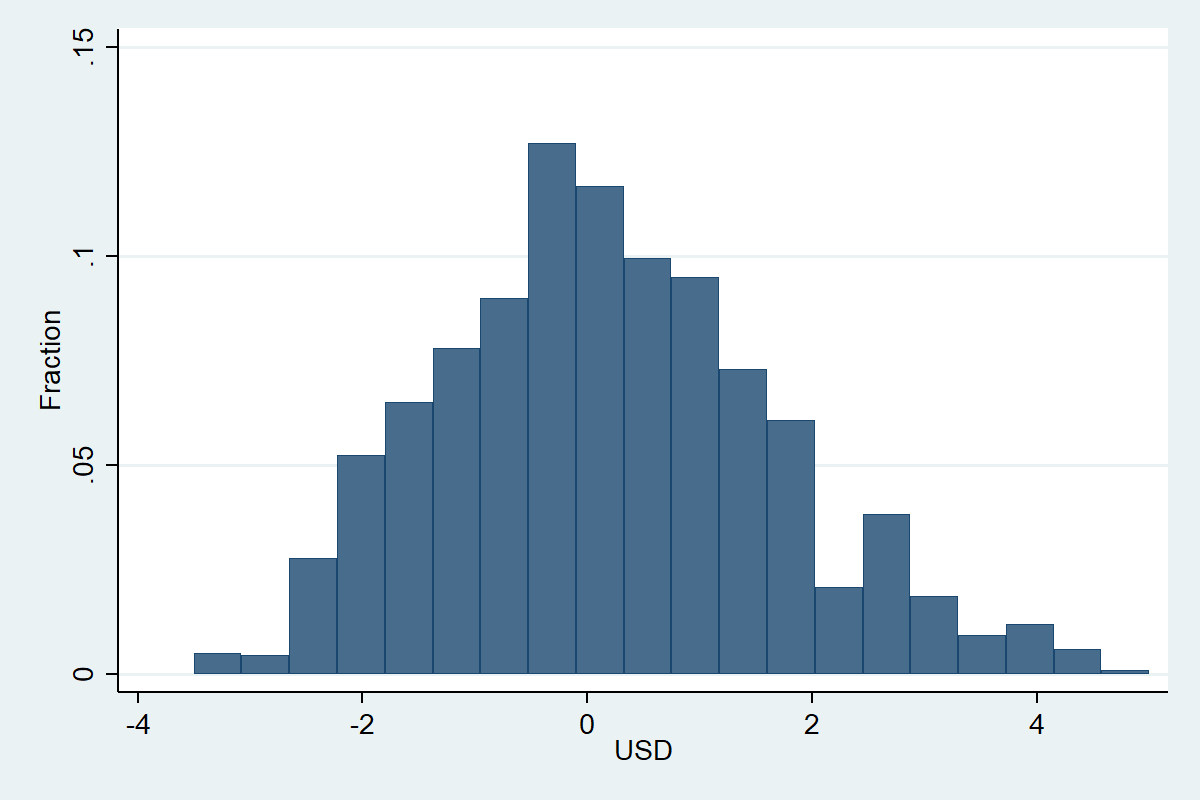
\includegraphics[width=.48\textwidth]{Graphs/hist_WTP_discr1_w.png}}
	\hfill
	\subcaptionbox{FP only}{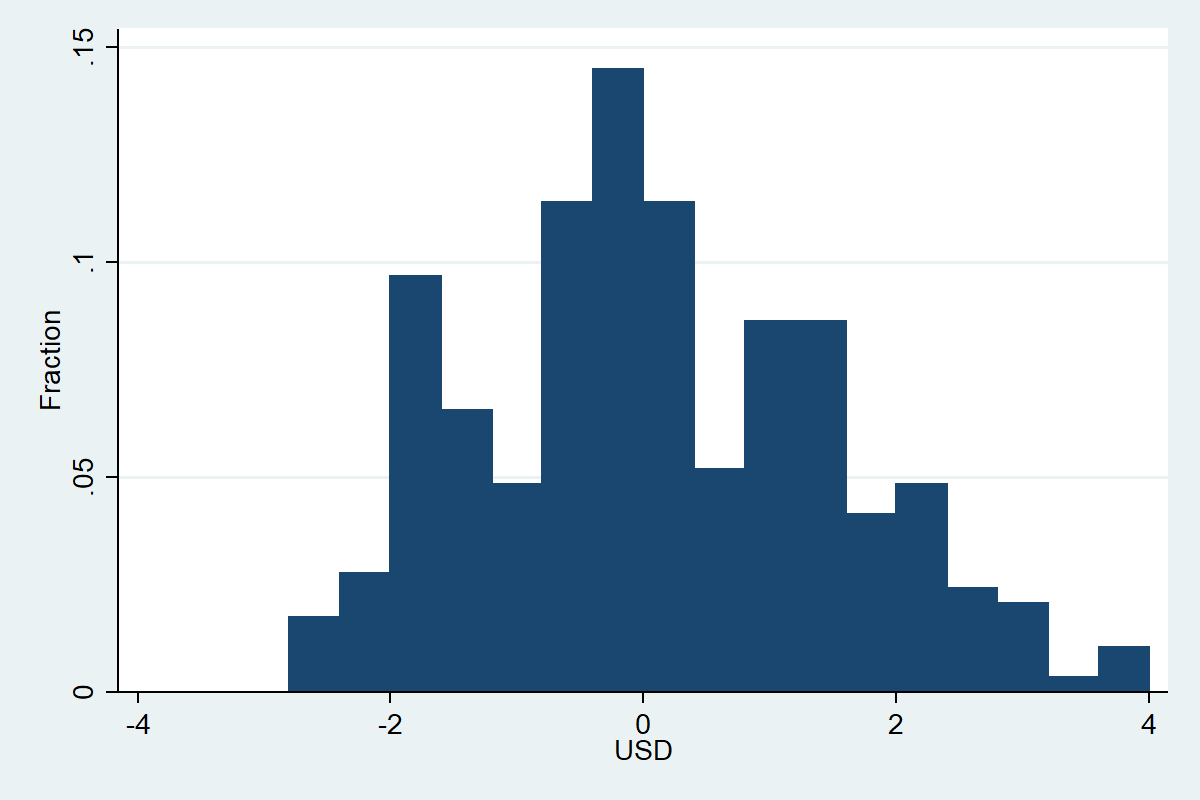
\includegraphics[width=.48\textwidth]{Graphs/hist_WTP_discr1fp.png}}
	\hfill
	\vspace{2em}
	\subcaptionbox{FN only}{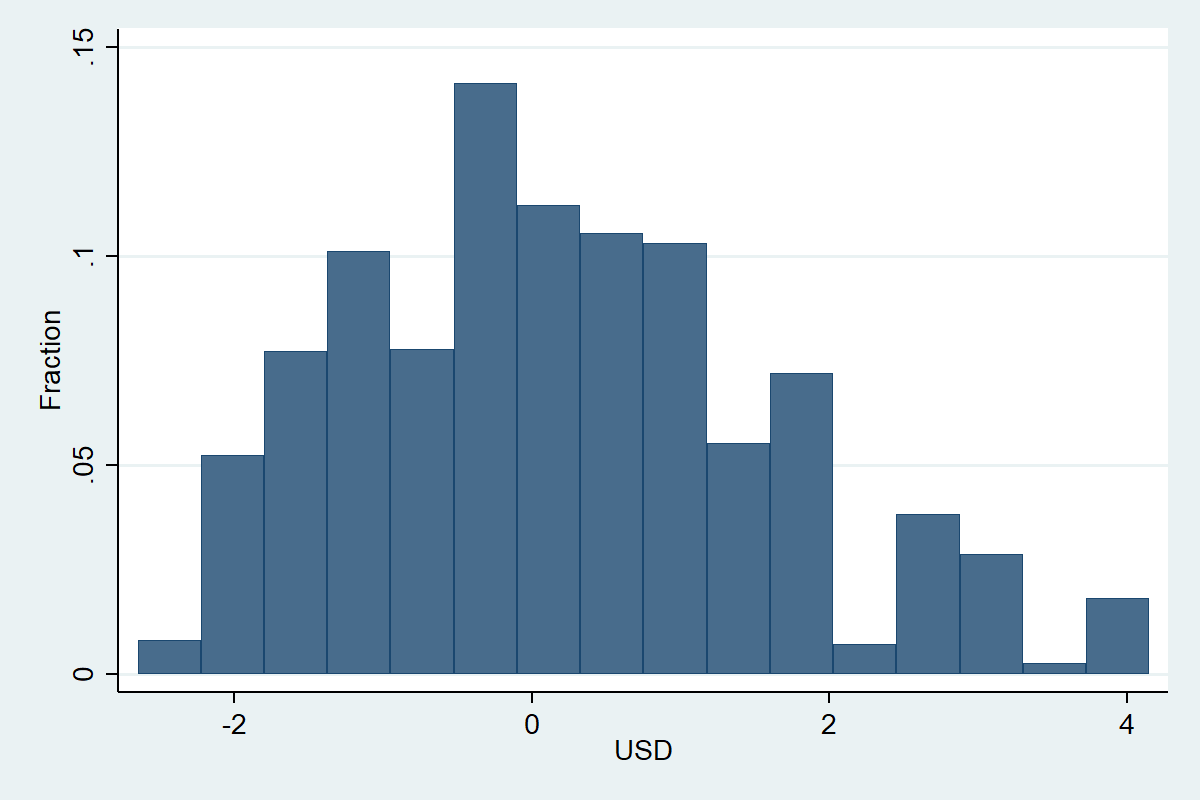
\includegraphics[width=.48\textwidth]{Graphs/hist_WTP_discr1fn_w.png}}
	\hfill
	\subcaptionbox{Both FP and FN}{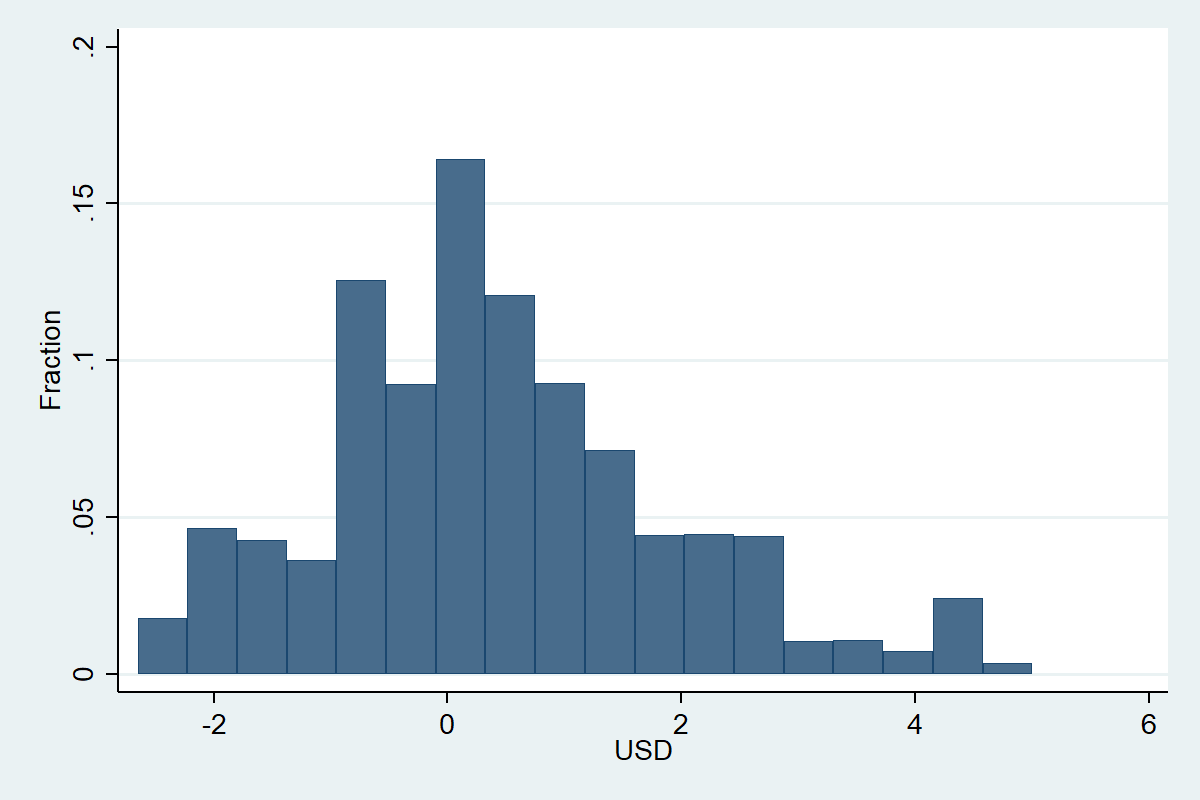
\includegraphics[width=.48\textwidth]{Graphs/hist_WTP_discr1fpfn_w.png}}
	\hfill
    \makebox[0.95\textwidth][l]{%
        \parbox{0.95\textwidth}{%
            \footnotesize\textit{Notes:} WTP Discrepancy is defined as Empirical WTP - Risk-Neutral WTP. Each observation is weighted by the inverse of its treatment frequency.
        }%
    }
\end{figure}


Our comparisons in Table~\ref{tab:wtpdis_by_stype} also do not find differences between the empirical WTP and the risk-neutral WTP for 3 out of 4 signal types: honest, FN-only, and FP-only. For signals from information structures with both FP and FN rates, however, the empirical WTP is significantly higher than the risk-neutral WTP. Subjects' overvaluations were similar for both low and high priors, but they are not statistically significant. Additionally, subjects tend to overvalue signals with positive FP-only rates in low-prior environments ($p \in \{0.1,0.2\}$) and undervalue signals in high-prior environments ($p \in \{0.3,0.5\}$).

Willingness-to-pay for signals increases with priors starting from \$0.86 on average when $\pi=0.1$ and reaching \$2.10 for the highest prior of 0.5. This stands in contrast to the theoretical value, which is largest for a prior of 0.3 (followed closely by the value for for a prior of 0.2). Hence subjects tend to overpay for signals with low priors and underpay for medium priors.

% \agt{\textbf{EITHER this para:}}

% \agt{When we break down these discrepancies by type of information structure (Table~\ref{tab:WTPnonpar}), we find that on average subjects: (i) undervalue completely truthful signals; and (ii) overvalue signals generated by a FN information structure, and signals generated from an information structure with a combination of FN and FP rates. In low-prior environments ($p \in \{0.1,0.2\}$), subjects overvalue signals from FP only and FP+FN information structures. In high-prior environments ($p \in \{0.3,0.5\}$), subjects undervalue truthful signal and signals generated from an FP information structure, and overvalue signals from an FN-only and FP+FN information structures.}   

% \agt{\textbf{OR the following alternative para:}}

% \agt{In Table~\ref{tab:WTPnonpar}, we present these discrepancies by type of information structure and prior. On average, subjects undervalue truthful signals and overvalue erroneous signals. Column 1 shows that the undervaluation of truthful signals primarily occurs in high-prior environments ($p \in \{0.3,0.5\}$). Column 2 shows that when the signal was generated by an information structure with an FN-only rate, subjects overvalue the signal in high-prior environments. However, column 3 suggest that when the signal was generated by an information structure with an FP-only rate, this discrepancy with the risk-neutral WTP varies with the prior: in low-(high-)prior environments, subjects over-(under-)value such signals. Finally, subjects consistently overvalue signals that were generated by an information structure with a combination of FN and FP rates (column 4).}   





%%%%%%%%%%%%%%%%%%%%%%%%%%%%%%%%%%%%%%%%%%%%%%%%%%%%%%%%%%%%%%%%%%%%%%%%%%%%%%%%%%%%%%%%%%%%%%%%%

\begin{table}[H]\centering \caption{Average WTP discrepancy (WTP-Value) by Signal Type} \begin{tabular}{ccccc} \hline \hline
\textbf{Priors}&\textbf{Honest}&\textbf{FN only}& \textbf{FP only} & \textbf{FP and FN}\\ \hline
All priors&-0.260&0.192&0.085&0.417\\
Low priors&-0.059&-0.011&0.609*&0.436\\
High priors ($>$0.2)&-0.461&0.395&-0.440&0.398\\
\hline \multicolumn{5}{l}{\footnotesize *The number of stars represents statistical significance (0.05, 0.01, 0.001)} \\ \end{tabular} \end{table}



\subsection{The Responsiveness of WTP to Error Costs} 

\begin{hypothesis}\label{hyp:eqSen} 
Subjects' preferences demonstrate equal sensitivity to the expected costs from false-positive and false-negative outcomes. 
\end{hypothesis}

\begin{result}
On average, we cannot reject the hypothesis of equal sensitivity. However, we observe significant heterogeneity with respect to priors: subjects tend to overvalue false-positive costs for low prior probability events and overvalue false-negative costs for high prior probability events.
\end{result}

Ultimately, we want to learn how people respond to the expected \textit{costs} from signals generated by different information structures and whether our simple theoretical model adequately captures this behavior. We therefore first examine whether and how subjects deviate from the benchmark WTP of our risk-neutral, Bayesian-updating, utility-maximizing agent. We then test whether these deviations can be explained by risk preference or updating accuracy. Finally, we describe our findings on the heterogeneous sensitivity of the WTP by prior --- which motivates our discussion on the potential mechanisms behind these deviations that we address in the next section.

We begin by estimating the relationship between the deviations of the empirical WTP from the benchmark model on FP and FN costs. The FP and FN costs studied here --- defined above as $\pi (1-P_{01})c$ and $\pi P_{01}L$ --- differ from their respective rates because they incorporate the cost associated with each error type. For example, a high false-negative rate imposes fewer costs when priors are low because the adverse outcome is already unlikely, whereas a high false-negative rate carries substantial costs when the prior probability of the adverse outcome is high. We estimate the following regression:
\[\Delta b_{is} = \beta_0 + \beta_1 FPC + \beta_2 FNC + \delta_i + \varepsilon_{is}\]
where $\Delta b_{is} = (b_{is} - b^*_s)$ is the difference between individual $i$'s WTP and the risk-neutral WTP for signal $s$, and FPC (FNC) is the false positive (false negative) cost. All specifications include subject fixed effects $\delta_i$, with standard errors clustered at the subject and treatment levels.

% Note here that false positive or false negative \textit{costs} are functions of both the rates and the costs of the consequences of those rates.  For example, a high false-negative rate imposes fewer costs when priors are low because the adverse outcome is already unlikely, whereas high false-negative rates carry substantial costs when the prior probability of the adverse outcome is high. All specifications include subject fixed effects, with standard errors clustered at the subject level. 


%%%%%%%%%%%%%%%%%%%%%%%%%%%%%%%%%%%%%%%%%%%%%%%%%%%%%%%%%%%%%%%%%%%%%%%%%%%%%%%%%%%%%%%%%%%%%%%%%


\begin{table}[htbp!]
\centering
\adjustbox{max width = \textwidth}{
	\begin{threeparttable}
	\caption{Deviations from Signal Value (WTP - Value) and Signal Characteristics}
	\label{tab:wtp_ols_cl}
	\begin{tabular}{l*{5}{c}}
		\hline\hline
		&\multicolumn{3}{c}{\multirow{2}{*}{All}} & \multicolumn{2}{c}{Prior}\\ \cmidrule(lr){5-6}
		&&&& $\{.1,.2\}$ & $\{.3,.5\}$\\ 
		\cmidrule(lr){2-4} \cmidrule(lr){5-5} \cmidrule(lr){6-6}  
		&\multirow{1}{*}{(1)} & \multirow{1}{*}{(2)} & \multirow{1}{*}{(3)} & \multirow{1}{*}{(4)} & \multirow{1}{*}{(5)}\\
	\hline
	\\ [-0.5em]
		\exInput{Tables/wtpdiff_ols_cl.tex}
				\hline
		Subject FE & Yes & Yes & Yes & Yes & Yes \\
		Inconsistent Risk Pref. Interactions & No & Yes & Yes & Yes & Yes \\
		Inaccurate Belief Interactions & No & No & Yes & Yes & Yes \\
		Prior Probability FE & No & No & No & Yes & Yes \\
		\hline\hline
	\end{tabular}
	\begin{tablenotes}[flushleft]
		\item\leavevmode\kern-\scriptspace\kern-\labelsep \small\textit{Notes:} Standard errors in parentheses (clustered by subject and treatment).  */**/*** indicates statistical significance at 10/5/1 percent. The bottom panel includes the total coefficient value estimates (baseline+interaction).
	\end{tablenotes}
	\end{threeparttable}
}
\end{table}		
		
%%%%%%%%%%%%%%%%%%%%%%%%%%%%%%%%%%%%%%%%%%%%%%%%%%%%%%%%%%%%%%%%%%%%%%%%%%%%%%%%%%%%%%%%%%%%%%%%%

Table~\ref{tab:wtp_ols_cl} reports the results of our regression. Column 1 presents the basic results that do not account for risk preference and belief accuracy. If subjects are risk-neutral expected-utility maximizers, we expect all coefficients to be jointly and individually insignificant. Instead, column 1 shows positive coefficients for both FP and FN costs, albeit only significant for the latter. As costs increase, subjects should downward-adjust their WTP accordingly. These positive coefficients show that relative to the risk-neutral benchmark, our subjects did not react enough to rising costs (by adjusting their WTPs), resulting in a WTP discrepancy that increases with costs.  

Theoretically, risk-neutral subjects value the marginal costs of false-negative and false-positive events symmetrically. Although column 1 shows that the coefficient on FN costs is slightly lower, the difference between the coefficients on FP and FN costs is not statistically significant.
% \aut{This difference albeit small \agt{XXX Alex: is this small? it's at least 50\% larger -- but is it economically small? XXX} is statistically significant at 5\% in our baseline estimation, and is more pronounced once we control for both risk aversion and belief accuracy (column 3)}. \agt{The smaller coefficient on FN costs suggests that, between FN and FP, WTPs tend to be more responsive --- i.e., they align more closely to the risk-neutral benchmark --- to increasing FN costs.}
 

% Theoretically, risk-neutral subjects should value the marginal costs of false-negative and false-positive events symmetrically \agt{XXX should we have an equation that shows this in the theory section then reference it here? XXX}. Table~\ref{tab:wtp_ols} however shows that the coefficient on FN costs is slightly lower \aut{(WTP sensitivity is larger)}  meaning a higher sensitivity to FN costs. \aut{This difference albeit small is statistically significant at 5\% in our baseline estimation, and is more pronounced once we control for both risk aversion and belief accuracy (column 3)}.

% To address the potential concern of WTP censoring both at zero and at the maximum bid of \$5, we also estimate the same relationship using a tobit regression (see Table~\ref{tab:wtp_tobit} in the Appendix). To make our results directly comparable we still use the difference between the elicited WTP and the theoretical value as the dependent variable and account for varying upper and lower bounds. We find that our essential results do not change: subjects under-react to FP and FN costs, and under-react to FP costs for low priors and to FN costs for high priors.

\paragraph{Risk Preference and Belief Accuracy}
% Our baseline estimation in column 1 indicates significant deviations from the behavior of a risk-neutral agent as predicted by the model. 
% The positive and significant coefficients suggest that these deviations are increasing in FP and FN costs. In other words, as signal quality deteriorates (with increasing FP or FN rates), our subjects do not reduce their valuation of the signals as quickly as a risk-neutral agent would.
% Column 1 documents deviations of subjects' WTP from the risk-neutral utility-maximizing benchmark. 
Since our benchmark model assumes both risk neutrality and perfect updating, the finding that our subjects do not adequately adjust their WTP to rising error costs  could arise from two channels. First, Proposition~\ref{thm:riskAverse2} suggests that risk preferences can influence the sensitivity of WTP to FP and FN rates. Second, systematic biases during updating can also cause deviations. 

We find that risk preferences affect the sensitivity to a signal's quality, but fall short in explaining the systematic WTP biases reported above. We use data from the BP task to categorize subjects by their risk preference. We classify all the subjects with internally consistent BP choices into three categories: risk averse, risk neutral, and risk loving.\footnote{We classify most subjects to risk-averse, risk-loving or risk-neutral based on the total number of protection choices made in the BP task, with 2 and 3 choices corresponding to risk-neutrality (protecting starting from 0.2 or 0.25).  Subjects that make more than one inconsistent choice in BP are included as their own category.} 

Column 2 explores the heterogeneity of subject responses to FP and FN costs by their risk preferences, with risk-neutral as the default category. The total coefficient values for risk-averse and risk-loving subjects, including their respective standard errors and $p$-values, are presented at the bottom panel. Among risk-neutral and risk-loving subjects, the WTP discrepancies increase with both FP and FN costs --- suggesting that they do not downward-adjust their WTP enough in the face of increasing error costs due to the lower signal quality. In contrast, the WTP discrepancies of risk-averse subjects are uncorrelated with rising error costs.

Subjects' under-reaction to deteriorating signal quality remains even after we further control for their ability to Bayesian update. We use data from the BE task to construct a measure of subjects' (posterior) belief accuracy.\footnote{We calculate a belief error as the absolute value of the difference between the subject's belief and the true posterior probability and then average these errors across all the decisions with identical priors, false positive, and false negative rates. A subject's posterior belief for a decision is defined as accurate if its error is less than the median error across all the subjects making the same decision.} Column 3 presents the most flexible specification that controls for belief accuracy and risk preference by including triple interactions of belief accuracy, risk preference, and signal characteristics. The baseline group is the group of risk-neutral subjects with relatively accurate beliefs. We find that subjects with more accurate beliefs are not more likely to adjust optimally to rising FP and FN costs on average.\footnote{Aside from these theoretically motivated individual differences, we investigate several other characteristics. Heterogeneity is not driven by demographic characteristics (e.g., age, gender) or prior statistical coursework.  The complete set of results are in Appendix Table~\ref{wtp_dem}.}
  
\paragraph{Heterogeneity by Prior} We motivate our experiment with a real-world problem of designing warning systems --- often for events with low probabilities. With a low prior, the default action of risk-neutral subject would be not to protect, and vice versa with a high prior. The signal would help risk-neutral subjects decide whether to maintain or switch away from the default action. We split the priors into two groups using the threshold of 0.25 (= protection cost/potential loss), and we incorporate prior-probability fixed effects to the aforementioned flexible specification. 

Column 4 of Table~\ref{tab:wtp_ols_cl} presents the results for low-prior WTPE tasks. For a low prior, i.e, $p \in \{0.1,0.2\}$, the WTP discrepancies of risk-neutral and risk-loving subjects from the risk-neutral benchmark increase with FP costs. These subjects do not optimally reduce their WTP enough as signal quality deteriorates, leading to the overvaluation of FP signals. Column 5 presents the results for high-prior WTPE tasks. With high priors, the WTP discrepancies of risk-neutral and risk-loving subjects once again increase with FN costs, leading to the overvaluation of FN signals. 

\bigskip

\begin{center} * * * \end{center}

\noindent To address the potential bias from WTP censoring both at zero and at the upper bound of \$5, we also estimate the same relationship using a tobit regression (see Appendix Table~\ref{tab:wtp_tobit}). To maintain comparability, we use the difference between the elicited WTP and theoretical value as the dependent variable and account for varying upper and lower bounds. We find that our essential results do not change: subjects underreact to FP and FN costs for all the priors on average, and underreact to FP costs for low priors and to FN costs for high priors.


% \agst{In summary, with low priors, subjects do not reduce their WTP enough to account for the deteriorating signal quality captured by the false-positive costs. In contrast, with high priors, they underreact to false-negative costs.}
% \agt{In practice, most warning systems are designed for low probability events. In such cases, users would tend to overpay for signals with high false-positive costs and underpay for signals with high false-negative rates. For example, they would prefer a smoke alarm that never misses fire incidents, even when its expected cost of false alarms is high. Risk preferences seem to affect this pattern, with risk-averse subjects' WTP tracking closer to the WTP of the risk-neutral benchmark.}\agst{, but most interaction coefficients are not statistically significant despite large magnitudes.}
% \pmt{I don't really think we want to close with this last sentence.  Arya's addition here is good, but do you think it belongs here?  Or should we use it as part of the conclusion?}\agt{Maybe move/drop the whole paragraph?}

\subsection{Understanding Source(s) of Empirical Deviations}\label{sec:discussion}

The under-reactions of subjects' WTP to FP (FN) costs for low (high) priors are inconsistent with our risk-neutral model. Equations~\ref{eq:dWTP_dFP} and~\ref{eq:dWTP_dFN} in Section~\ref{sec:model} suggest that WTP should respond more to FP rates (relative to FN rates) for low priors and vice versa for high priors. That is, for a given FN rate, false negative outcomes are much less likely with low priors and hence impose lower costs on the agent. As priors increase, FN rates become more salient while FP rates become less salient. Instead, our subjects react very similarly to FP and FN rates for both low and high priors.



\begin{figure}[H]
\centering
\caption{Theoretical and Estimated WTP Sensitivities to Error Rates by Prior} \label{fig:Comparison}
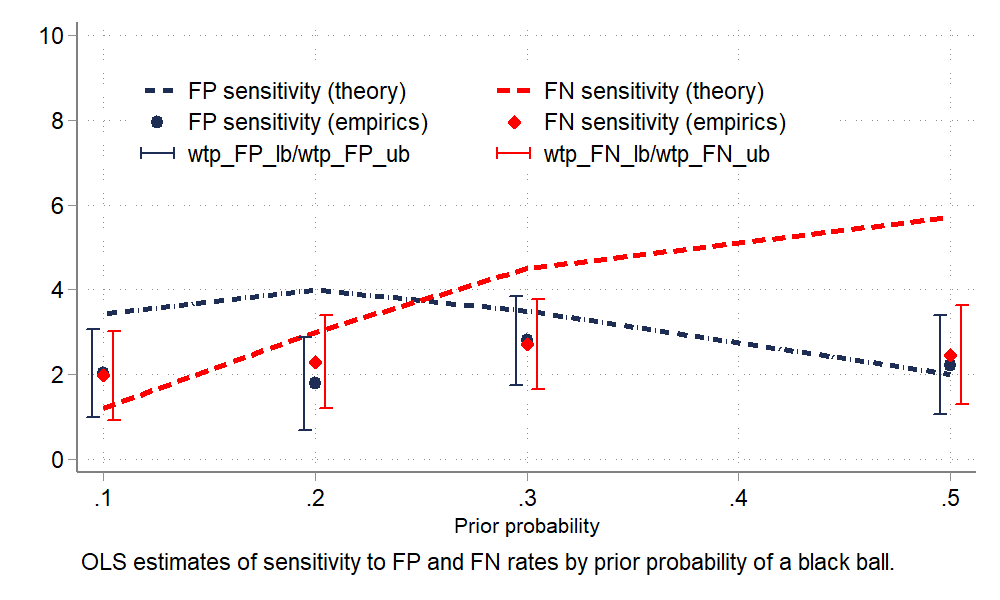
\includegraphics[width=0.8\textwidth]{Graphs/sensit_comparison.png}
\end{figure}


\bigskip

To illustrate, we obtained the sensitivities of WTP on FP and FN rates by estimating the following regression for each prior for the elicited WTP ($b^*$):
\begin{equation}
\label{eq:tobit}
b^* = \alpha+\beta_{FP} FP +\beta_{FN} FN+\epsilon
\end{equation}
In Figure~\ref{fig:Comparison}, we overlay these estimates on the line plots of the theoretical sensitivities of WTP on FP and FN rates across different priors (based off Equation~\ref{eq:tobit}).\footnote{Given that theoretical sensitivities depend on information structures which are pooled within priors, we fit the same regression to the theoretical values and report coefficients as theoretical sensitivities. With tobit estimates, the empirical coefficients are generally higher but are also very close to each other and follow the same pattern.  However, we cannot fit them easily for the theoretical values.} The figure shows that the point estimates of the sensitivity coefficients of WTP on FP rates for lower priors ($p \in \{0.1, 0.2\}$) are below their theoretical benchmarks. In contrast, the point estimates of WTP sensitivity on FN rates for higher priors ($p \in \{0.3, 0.5\}$)  are significantly below. Surprisingly, across all priors, the empirical estimates of the sensitivities on FP and FN rates are very close to each other.

% Figure~\ref{fig:Comparison} illustrates this puzzling behavior. This figure plots estimates from \agt{Tobit} regressions of reported WTP --- instead of its deviation from the risk-neutral WTP --- on FP and FN rates. \agt{We overlay these estimates on the plots of the theoretical WTP sensitivity to changes in FP and FN rates across priors (based on Equation XX).} We find that the sensitivities of subjects' WTP to both FP and FN rates increase with priors and that the change occurs relatively smoothly, and the two sensitivities are also surprisingly close to each other.\footnote{We cannot reject the hypothesis that two sensitivities are equal to each other for any of the priors.} 

We consider six candidate explanations for these puzzling results: (i) risk preferences; (ii)probability weighting; (iii)  anchoring; (iv) valuing non-instrumental information; (v) the anticipation of bias in the protection decision; and (vi) a failure to distinguish how FP and FN error rates ought to affect calculated posteriors differently. 


\paragraph{Risk Preferences.} Our evidence suggests that risk preferences do not explain this behavior. We test the risk preference hypothesis using subjects' BP choices. Columns 4 and 5 of Table~\ref{tab:wtp_ols_cl} already show that, even after controlling for subjects' risk preferences, the coefficients on FP and FN costs remain very different for low and high priors.  We augment this analysis by explicitly testing for interactions between risk-preferences, priors, and FP and FN rates (Appendix Table~\ref{tab:wtp_risk}). We find that these interactions are mostly insignificant, except for the interactions between FN rates and risk aversion in low-prior environments. The heterogeneity largely remains after controlling for risk preferences, but the interaction between high priors and FP rates becomes insignificant.

\paragraph{Probability Weighting.} Rank-dependent probability weighting assumes that subjects evaluate lotteries using transformed outcome probabilities that account for the preference ranking of each outcome and cumulative probability distribution.  It helps to explain extreme low probability outcomes receiving disproportionate weight in decision-making \citep{quiggin_theory_1982} and hence is applicable to protection decisions in which losses can be both rare and extreme.

Assuming that each lottery $p$ has ordered outcomes $x_1\succ x_2 \succ...\succ x_n$ with probabilities $p_i$ for the outcome $i$, rank-dependent utility re-weights cumulative probabilities of each outcome using a weighting function $\phi:[0,1]\to[0,1]$ in the following way:

\[U(p) = \phi(p_1)u(x_1)+\sum_{i=2}^n \left(\phi\left(\sum_{j=1}^i p_j\right)-\phi\left(\sum_{j=1}^{i-1}p_j\right) \right)u(x_i) \]


As follows from the equation, the weights depend on the ranking of the outcomes and the probabilities within each lottery. In the signal purchase decision,  subjects compare a simple blind protection lottery with the compound lottery of first drawing a signal and then choosing a trivial protection outcome or a simple no protection lottery with a signal. We assume that the reduction of compound lotteries applies so that the compound lottery of informed protection is ranked equivalently to a reduced simple lottery with weighting applied to all the possible outcomes. This means that the utility with a signal can be written as:

\[ U_S = \phi(\pi P_{01})u(Y-b-L)+[\phi((1-\pi)P_{10}+\pi P_{11})-\phi(\pi P_{01})]u(Y-b-c)+\]
\[+[1-\phi((1-\pi)P_{10}+\pi P_{11})-\phi(\pi P_{01})]u(Y-b)\]

After applying implicit differentiation by FP and FN rates we obtain that the ratio of sensitivities to FN and FP rates should satisfy:
\begin{equation}
{db / dP_{01}  \over db / dP_{10}} = {\pi \over (1-\pi)} \Bigl({\phi'(\pi P_{00}) \over \phi'(\pi+(1-\pi)P_{10})}\Bigr) {(u(Y-c-b)-u(Y-L-b))\over (u(Y-b)-u(Y-c-b))}
\end{equation}


Probability weighting with reasonable parameter choices can explain higher relative sensitivity to FN costs when the priors are low, though it does not explain lower relative sensitivity when the priors are high. First, note that this ratio is equivalent to the expression we derived for the EU maximizers in the general case, except the additional multiplier $\Lambda\equiv \Bigl({\phi'(\pi P_{00}) \over \phi'(\pi+(1-\pi)P_{10})}\Bigr)$ which is equal to a ratio of derivatives of the weighting functions at two different points. We know that $\pi P_{01}<\pi<\pi+(1-\pi)P_{10}$ and that, for our experimental parameters, $\pi+(1-\pi)P_{10}\leq 0.75$ meaning that the value is still likely to fall in the mid-range of an S-shaped weighting function. Thus, for small priors $\pi$ or for small FN rates $P_{01}$, we have $\Lambda>1$, implying higher relative sensitivity to FN rates. For higher priors and FN rates $\Lambda$ would be closer to one making little difference in relative sensitivity\footnote{\citet{gonzalez_shape_1999} report very diverse estimates of shapes of weighting functions estimated individually for 10 subjects. We calculate the ratio using linear in odds probability weighting function for all their parameter estimates and find that the ratio is greater than one for all our treatments except the treatment with prior $\pi=0.5$ and the FN rate of 0.5. Using their power weighting function estimates produces ratios which are always greater than one.}.

\paragraph{Anchoring.} The evidence also does not support the hypothesis that anchoring on previous priors explains higher sensitivity to FN rates for low priors. The prior order is randomized with some subjects starting with lower priors and other starting with higher priors. Most subjects (159 out of 206) also change their reported WTP when facing a new prior in round 4, demonstrating responsiveness to information on priors. The average belief error in the BE task is actually \emph{lower} for the second set of priors rather than the first (0.201 vs 0.186), which suggests that changing priors does not make subjects more confused. Most importantly, our main results on WTP sensitivity hold even when we limit the sample only to the first prior in each sequence.

\paragraph{Non-instrumental information.} There is evidence in the literature of people valuing ``non-instrumental information'' that does not affect their decisions. For example, \citet{eliaz_paying_2010} find that subjects are willing to pay to know the probability of their choice being correct even if this information cannot affect their choice, while \citet{ganguly_fantasy_2017} document that most people are willing to pay a small amount to know their pre-determined experimental payoffs at the beginning of the experiment rather than at the end.  Similarly, \citet{Masatlioglu2023} reveal a strong and systematic preference for positively skewed information, even when such signals are less informative, suggesting that anticipatory emotions such as hope and anxiety shape information demand independently of instrumental value.\footnote{Unlike \citet{Masatlioglu2023}, \citet{OliverosZultan2025} find that decision makers exhibit a striking and persistent preference for symmetric sources, i.e., those offering a balanced distribution of positive and negative signals, even when asymmetric sources would yield more decision-relevant information.  The authors argue that symmetry exerts an intrinsic appeal, suggesting that individuals prefer information structures that “feel fair” or representative, independent of their actual informativeness.} 
Most information in our experiment is instrumental by design, i.e., it informs their choices, and indeed enters into subjects' decisions as evidenced by choices in the IP task. Nonetheless, many subjects have a positive WTP for signals that cannot affect their IP decisions (295 out of 1242 total choices). It is therefore plausible that the reported WTPs include some non-instrumental components. 

Preferences for non-instrumental information cannot, however, provide a full explanation of our results, mainly because there is no time delay between receiving a signal and learning the outcome.  If the WTP task round is selected as a payment round, the subject receives a signal, chooses an action, and then immediately learns their payoffs.  This leaves essentially no window for anticipatory feelings assumed to be the causal mechanism behind the demand for non-instrumental information in most of the literature. Additionally, the closeness of coefficients for FP and FN rates also seems a priori implausible based only on the non-instrumental information value story because, in contrast to our last explanation, no theory of preferences for non-instrumental information suggests the effects should be so similar to one another.

\paragraph{Anticipation of Bias in Protection Decision.} Since both IP and WTP task responses exhibit certain unexpected biases, subjects might adjust their bids in the WTP task in anticipation of the projected distortions in their use of the signal in the IP task. For example, a subject expecting to always protect for a particular information structure might report a lower WTP. This should be expected if subjects make consistent choices across tasks. We find that their IP biases do affect their bids, but fail to explain the main patterns of sensitivities to FP and FN costs that we observe.

To show this, we define two variables measuring the discrepancies in expected payoffs due to elicited strategies in IP ($a_{iw}, a_{ib}$) and BP tasks ($a_{i}$) versus optimal decisions for a risk-neutral decision-making $(a^*_i, a^*_{ib}, a^*_{iw})$. The first variable measures the protection-cost component and the second variable the loss component of the shortfall in the value of the signal under the subject’s elicited strategies relative to the optimal benchmark\footnote{Given that there is no elicited blind protection choice for prior of $\pi=0.5$, we assume full protection. For context, 65\% of subjects protect for the highest prior probability of 0.3 in our BP elicitation.}:

\[
\Delta^{\text{prot}}_{i}\equiv c\Big\{(a_i-a^*_i)-\big[P(S=W)(a_{iw}-a^*_{iw})+P(S=B)(a_{ib}-a^*_{ib})\big]\Big\}
\]

\[
\Delta^{\text{loss}}_{i}\equiv \pi L\Big[(a^*_i-a_i)-\big(P_{11}(a^*_{iw}-a_{iw})+P_{01}(a^*_{ib}-a_{ib})\big)\Big]
\]

Here $P(S=B)=\pi P_{11}+(1-\pi)P_{10}$ is the probability of a black signal, and $P(S=W)=\pi P_{01}+(1-\pi)P_{00}$ is the opposite. The sum of these two variables equals a decrease in the signal's value for a risk-neutral subject if using actual subject $i$ strategies. Defining the expected benefit in this way allows for an asymmetry in responding to large losses versus relatively small protection costs. 

Appendix Table A10 reports the estimation results of the deviation of the empirical WTP from the signal value (similar to Table~\ref{tab:wtp_ols_cl}) with the two new measures of bias in informed protection decisions. The coefficients on the added covariates are statistically significant but relatively small in magnitude. At the same time, both coefficients on FP costs for low priors and FN costs for high priors remain highly statistically significant. Thus, we conclude that subjects' biases in how they will utilize signals when facing an IP task do not explain the observed pattern of sensitivities to FP and FN rates.

\paragraph{Failure to distinguish between FP and FN} Instead, we argue that the observed sensitivity patterns emerges because many subjects neglect the difference between FN and FP rates, treating these two characteristcs as if they were the same thing. Subjects' own proffered explanations motivate our consideration of this possible mechanism.  At the end of the experiment, we asked subjects to explain to us how they made their protection choices.\footnote{The text of all the responses are in the appendix.} Out of 206 subjects, 70 refer to the \emph{percentage}  or presence of dishonest gremlins as their rationale for choosing protection. For example:
\begin{itemize}
	\item ``\emph{my strategy for this task was to only buy protection if there was a white or black gremlin and not if there was a truth gremlin}''
	\item ``\emph{If there were only honest gremlins then I never protected but even if there was one white-swamp gremlin or one black-swamp gremlin then I payed} (sic) \emph{for protection.}''
\end{itemize}

Among the other 136 subjects, some may use this heuristic without describing it and many subjects make decisions solely based on priors.\footnote{Several studies find that decision makers use heuristics in choice environments like this.  For example, \citet{MontanariNunnari2023} investigate selective exposure to information in an environment where two biased information sources differ in direction and reliability and find deviations from Bayesian rationality including reliance on simple heuristics such as ``listen to the more reliable source."  Similarly, \citet{CharnessOpreaYuksel2021} study how individuals choose between two information sources with opposing biases when forming beliefs about a binary state and find that subjects rely on intuitive, but flawed, heuristics about which sources are more “useful.”} The similarity of the coefficient estimates for FP and FN rates for each prior as reported in Figure~\ref{fig:Comparison} is consistent with these statements. If subjects neglect the difference between FP and FN risks when choosing their WTP, it would explain both the coefficients' similarity and the lack of variation with respect to priors in Figure~\ref{fig:Comparison}. Indeed, if subjects treat FP and FN rates the same and consider only the total proportion of false signals, they would assign equal weights to each of them, and the best-fit line of the signal value on the sum of FP and FN rates should be relatively flat because priors affect FP and FN costs in opposite ways.\footnote{The equality of coefficients on FP and FN rates is a necessary prediction of this explanation, but it can also emerge by chance with (some) heterogeneous risk preferences and probability weighting.}

We can test this hypothesis using choices from the BE and IP tasks when signals come from information structures that are obviously irrelevant in the wake of the signal. If subjects systematically neglect the difference between FP and FN rates, we expect subjects to (unexplainably) react to irrelevant information structures that would not have affected posteriors, namely that subjects would still react to FP (FN) rates when given a white (black) signal. This could happen if subjects react to FP rates as if they are FN rates, and vice versa. If present, this pattern cannot be explained by any of the aforementioned mechanisms.  

%%%%%%%%%%%%%%%%%%%%%%%%%%%%%%%%%%%%%%%%%%%%%%%%%%%%%%%%%%%%%%%%%%%%%%%%%%%%%%%%%%%%%%%%%%%%%


\begin{table}[htbp]\centering 
\caption{Updating Errors in BE Task} 
\label{updateErrorReg}
\adjustbox{max width=\textwidth}{
	\begin{threeparttable}
	\begin{tabular}{l*{3}{c}}
	\hline\hline
									&\multirow{2}{8ex}{\centering All}&\multicolumn{2}{c}{Signal Received}\\ \cmidrule{3-4}
									&&\multicolumn{1}{c}{White}&\multicolumn{1}{c}{Black}\\
									&\multicolumn{1}{c}{(1)}&\multicolumn{1}{c}{(2)}&\multicolumn{1}{c}{(3)}\\
	\hline

	
FP rate         &    0.797\sym{***}&    0.532\sym{***}&    1.063\sym{***}\\
                &  (0.069)         &  (0.051)         &  (0.127)         \\
FN rate         &   -0.243\sym{***}&    0.042         &   -0.528\sym{***}\\
                &  (0.060)         &  (0.057)         &  (0.101)         \\

Constant        &   -0.058\sym{***}&    0.328\sym{***}&   -0.444         \\
                &  (0.011)         &  (0.017)         &      (.)         \\
\hline
Observations    &     2460         &     1230         &     1230         \\
Adjusted \(R^{2}\)&    0.203         &    0.407         &    0.543         \\
	\\ [-1em]
	\hline
	Subject FE      &      Yes         &      Yes         &      Yes         \\
	\hline\hline
	\end{tabular}
	\begin{tablenotes}[flushleft]
			\item\leavevmode\kern-\scriptspace\kern-\labelsep \footnotesize \textit{Notes:} Standard errors in parentheses (clustered at the subject and treatment level). */**/*** indicates statistical significance at 10/5/1 percent.
	\end{tablenotes}								
	\end{threeparttable}
	}
\end{table}


%%%%%%%%%%%%%%%%%%%%%%%%%%%%%%%%%%%%%%%%%%%%%%%%%%%%%%%%%%%%%%%%%%%%%%%%%%%%%%%%%%%%%%%%%%%%

Table~\ref{updateErrorReg} presents the results from linear regressions of updating error (i.e., belief - posterior) on FP and FN rates by signal color with individual fixed effects to control for updating biases. Consistent with our conjecture, we observe that the FP rate has a significant positive effect on the error when the signal is \textit{white}, and that the FN rate has a significant negative effect when the signal is \textit{black}. 

To further explore this hypothesis, in Table~\ref{tab:protectReg}, we regress IP decisions on FP and FN rates and flexible controls of both posteriors and reported beliefs:\footnote{Given that the true functional form is unknown, we use a linear probability model to get unbiased coefficient estimates.}

	\[Prob(s_{ij}=1)=\alpha_i+\beta_1 P_{10}+\beta_2 P_{01} +Z(P_{ij})+Z(\mu_{ij})+\epsilon_{ij} \]
Here $s_{ij}$ is the protection decision of subject $i$ in treatment $j$, $\alpha_i$ is subject FE, $P_{10}$, $P_{01}$ are FP and FN rates, and $Z(P_{ij})$ and $Z(\mu_{ij})$ are the splines of FP or FN rates  and reported beliefs $\mu_{ij}$ to control for these variables in a flexible way. Each spline is a function $Z(x)$ which is just linear $x+C$ within one interval, and constant everywhere else. The splines are constructed so that their linear intervals cover the whole domain of probabilities and beliefs $[0,1]$.\footnote{We use Stata's \texttt{mkspline} command to create 5 splines $z_1(x),z_2(x),..z_5(x)$ of initial variable $x$ over the range $[0,1]$ such that $z_k(x)=\min[0,x-x_{k-1},x_k-x_{k-1}]$ with $x_k$ being equally spaced knot values. Splines account for potential nonlinear effects of posteriors and beliefs on protection decision with limited effect on degrees of freedom.} Columns 1 and 2 include only the flexible controls of the true posteriors. Columns 3 and 4 add further flexible controls to account for subjects' (often incorrect) beliefs, inferred from their BE responses.

Columns 1 and 2 show that, even after we condition on posterior and subject FEs that account for risk preferences, IP choices still changed with FP and FN rates. Notably, we find that FP rates increase the tendency to overprotect for a white signal. The effect remains after allowing for heterogeneity of sensitivities to FP and FN rates with respect to priors (Column 2). Columns 3 and 4 show that adding flexible controls for subjects' beliefs reduces the coefficient magnitudes, but they remain statistically significant. This suggests that beliefs offer only a partial explanation to these protection anomalies.

%%%%%%%%%%%%%%%%%%%%%%%%%%%%%%%%%%%%%%%%%%%%%%%%%%%%%%%%%%%%%%%%%%%%%%%%%%%%%%%%%%%%%%%%%%%%%
\begin{table}[htbp]\centering 
\caption{Informed Protection Response} 
\label{tab:protectReg}
\adjustbox{max width=\textwidth}{
	\begin{threeparttable}	
	\begin{tabular}{l*{4}{c}}
	\hline\hline
									&\multicolumn{1}{c}{(1)}&\multicolumn{1}{c}{(2)}&\multicolumn{1}{c}{(3)}&\multicolumn{1}{c}{(4)}\\
	\hline
		
		FP rate x (S=White)&    0.895\sym{***}&    0.943\sym{***}&    0.525\sym{***}&    0.571\sym{***}\\
                &  (0.089)         &  (0.093)         &  (0.095)         &  (0.098)         \\
FN rate x (S=White)&    0.537\sym{***}&    0.532\sym{***}&    0.307\sym{**} &    0.299\sym{**} \\
                &  (0.145)         &  (0.146)         &  (0.144)         &  (0.146)         \\
FP rate x (S=Black)&   -0.032         &    0.025         &   -0.065         &   -0.000         \\
                &  (0.201)         &  (0.204)         &  (0.196)         &  (0.202)         \\
FN rate x (S=Black)&    0.103         &    0.069         &   -0.005         &   -0.021         \\
                &  (0.074)         &  (0.080)         &  (0.087)         &  (0.093)         \\
S=Black         &    0.531\sym{***}&    0.542\sym{***}&    0.383\sym{***}&    0.374\sym{***}\\
                &  (0.103)         &  (0.114)         &  (0.105)         &  (0.115)         \\
p$>$0.2         &    0.039\sym{**} &    0.041\sym{**} &    0.024         &    0.029         \\
                &  (0.016)         &  (0.021)         &  (0.015)         &  (0.020)         \\
FP rate x (p$>$0.2)&                  &   -0.081         &                  &   -0.085         \\
                &                  &  (0.076)         &                  &  (0.079)         \\
FN rate x (p$>$0.2)&                  &    0.088         &                  &    0.048         \\
                &                  &  (0.099)         &                  &  (0.093)         \\
\hline
N               &     2424         &     2424         &     2424         &     2424         \\
Pseudo R-squared&    0.505         &    0.505         &    0.538         &    0.539         \\
Log-likelihood  & -830.188         & -829.168         & -773.731         & -773.018         \\

	
	\\ [-1em]
	\hline
	Subject FE & Yes & Yes & Yes & Yes \\
	Flexible controls for: \\
	\hspace{1.5ex} Posterior & Yes & Yes & Yes & Yes \\
	\hspace{1.5ex} Beliefs & No & No & Yes & Yes \\	
	\hline\hline
	\end{tabular}
	\begin{tablenotes}[flushleft]
			\item\leavevmode\kern-\scriptspace\kern-\labelsep \footnotesize \textit{Notes:} Coefficients are average marginal effects. Standard errors in parentheses (clustered at the subject level). */**/*** indicates statistical significance at 10/5/1 percent.
	\end{tablenotes}								
	\end{threeparttable}
	}
\end{table}



Overall, we observe a striking uniformity in sensitivity of WTP to both FP and FN rates. This pattern is consistent with subjects neglecting the difference between FP and FN signals, a behavior that is supported by subjects' explanations of their decision making and the anomalous sensitivities to FP and FN rates in other treatments in which they do not affect posterior probabilities.\footnote{This pattern is consistent with greater bias in belief elicitation when subjects have to engage in contingent reasoning versus smaller belief biases when eliciting responses after presenting a signal results, as \citet{aina_contingent_2023} found. This result implies that decisions to acquire information, such as decisions made in our experiment where subjects determining their WTP have to reason through contingencies, might suffer from persistent inherent biases. Indeed, we find that subjects commit reasoning errors which reduces the correlation between their WTP for a signal and its usefulness for decreasing expected potential costs.} 

\vspace{10pt}
\section{Conclusion}\label{sec:conclusion}

We study how information structures affect valuation of a warning signal. While the risk-neutral benchmark model does a good job of describing the average elicited WTP, it masks an important underlying heterogeneity.  Relative to the risk-neutral WTP, individual valuations of warning signals inadequately adjust for declining signal quality as false-positive (false-negative) costs increases for low (high) prior probability events. These deviations can be partly explained by risk preferences and the inability of subjects to discriminate between false-negative and false-positive errors. Probability weighting might also play a role in the case of low priors.

Our findings have direct applications for the design of warning signals. Bias in preferences for signals arising from risk aversion means that prioritizing false-negative outcomes while designing warning signals can be welfare enhancing, even when it increases the expected costs of using the signal. At the same time, finding ways to better present the signal's information structure to help users discriminate between false-positive and false-negative payoffs should improve individual decision making. Studies on Bayesian updating, for instance, show that medical professionals make better decisions if information on medical tests is presented in the form of expected frequencies rather than as a tuple of prior conditional probabilities \citep{hoffrage_natural_2015, mcdowell_meta-analysis_2017}.

Understanding the source of this asymmetry can also help reduce externalities associated with signal (mis)use. We find that people overvalue signals with excessive false alarms for a typical case with low-probability events. In some cases, individuals may not incur the full cost of false positive signals.  For example, the cost of medical overtreatment from tests with high false positives may be an externality absorbed by the healthcare system.  Similarly, first responders may be required by law to respond to automatic fire alarms installed in commercial buildings resulting in excess costs borne by taxpayers when false positive rates are high. 

Future research should also explore the role of warning signals as an experience good, to wit, how prolonged exposure to a signal with a given information structure can influence individual biases. For example, buying a smoke alarm that never misses may seem like a good idea at first, but may seem less so after a year experiencing repeated false alarms. Given our finding of insufficient attention to false-positive costs for rare events, ex-ante preferred warning signals could later be considered overly sensitive and ignored, leading to \emph{alarm fatigue} and increasing the risk of potentially preventable disasters.
% As we do not study how preferences change with experience, this constitutes another fruitful direction for future research.

% Aside from the direct implications for signal design and presentation, another interesting issue is conceptualizing a signal as an experience good.  That is, how does prolonged exposure to a signal with a given information structure influence the biases in subjects' preferences? For example, buying a smoke alarm that never misses fires may seem like a good idea at first, but may seem less so after a year experiencing repeated false alarms. Given that we observe insufficient attention to false-positive costs for rare events, there is a possibility that warning signals preferred ex ante would be considered overly sensitive and ignored later. As we do not study how preferences change with experience, this constitutes another fruitful direction for future research.


\vspace{20pt}
%%%%%%%%%%%%%%%%%%%%%%%%%%%%%%%%%%%%%%%%%%%%%%%%%%%%%%%%%%%%%%%%%%%%%%%%%%%%%%%%%%%%%%%%%%%%%



\clearpage

\bibliographystyle{aea}
\bibliography{Alerts4.bib,Nytimes_cancer.bib}


%%%%%%%%%%%%%%%%%%%%%%%%%%%%%%%%%%%%%%%%%%%%%%%%%%%%%%%%%%%%
% APPENDIX
%%%%%%%%%%%%%%%%%%%%%%%%%%%%%%%%%%%%%%%%%%%%%%%%%%%%%%%%%%%%

\begin{appendices}
\appendix
\setcounter{table}{0}
\setcounter{figure}{0}
\renewcommand{\thetable}{\thesection\arabic{table}}
\renewcommand{\thefigure}{\thesection\arabic{figure}}
\newpage


\section{Tables and Figures}


\begin{table}[h!]
\centering
\caption{Demographic Characteristics of Subjects} \label{summ_tab}
	\input{Tables/demography.tex}
\end{table}


\begin{table}[H]\centering
\caption{Average Protection by Signal Type and Prior}
\label{tab:nonparIP_A}
\adjustbox{max width=\textwidth}{
\begin{threeparttable}
\begin{tabular}{ccccccccc}
\hline\hline
\multirow{4}{6ex}{\centering \textbf{Row}}
& \multirow{3}{10ex}{\centering \textbf{Prior}}
& \multicolumn{2}{c}{\centering \textbf{Signal Characteristics}}
& \multirow{3}{12ex}{\centering \textbf{Signal}}
& \multirow{3}{10ex}{\centering \textbf{Posterior}}
& \multirow{3}{12ex}{\centering \textbf{Share Protect}}
& \multirow{3}{12ex}{\centering \textbf{Share Optimal}}
& \multirow{3}{8ex}{\centering \textbf{$p$}} \\
\cmidrule(lr){3-4}
& & \multirow{2}{12ex}{\centering \textbf{False Positive}}
  & \multirow{2}{12ex}{\centering \textbf{False Negative}}
  & & & & & \\
\\
& (1) & (2) & (3) & (4) & (5) & (6) & (7) & (8) \\
\hline
(1)&Low&No&No&White&0.000&0.034&0.000&0.111\\
(2)&Low&No&Yes&White&0.055&0.184&0.000&0.001\\
(3)&Low&Yes&No&White&0.000&0.290&0.000&0.003\\
(4)&Low&Yes&Yes&White&0.051&0.334&0.000&0.002\\
(5)&Low&No&No&Black&1.000&0.806&1.000&0.074\\
(6)&Low&No&Yes&Black&1.000&0.852&1.000&0.003\\
(7)&Low&Yes&No&Black&0.357&0.778&0.750&0.863\\
(8)&Low&Yes&Yes&Black&0.387&0.873&0.833&0.812\\
(9)&High&No&No&White&0.000&0.064&0.000&0.070\\
(10)&High&No&Yes&White&0.183&0.294&0.125&0.312\\
(11)&High&Yes&No&White&0.000&0.269&0.000&0.000\\
(12)&High&Yes&Yes&White&0.169&0.492&0.167&0.079\\
(13)&High&No&No&Black&1.000&0.844&1.000&0.022\\
(14)&High&No&Yes&Black&1.000&0.865&1.000&0.001\\
(15)&High&Yes&No&Black&0.667&0.840&1.000&0.007\\
(16)&High&Yes&Yes&Black&0.689&0.894&1.000&0.007\\

\\[-1em]
\hline\hline
\end{tabular}

\begin{tablenotes}[flushleft]
\item\footnotesize \textit{Notes: Column (8) reports the p-value for the test of equality between the theoretical prediction (Share Optimal) and the observed share of protection (Share Protect). Priors are grouped as low ($p \in \{0.1,0.2\}$) v. high ($p \in \{0.3,0.5\}$).}
\end{tablenotes}
\end{threeparttable}
}
\end{table}


\begin{table}[h!]\centering 
\caption{Error Decomposition} 
\label{belief_decomposition}
\adjustbox{max width=\textwidth}{
	\begin{threeparttable}	
	\input{Tables/table_be3_AU_cl.tex}
	\begin{tablenotes}[flushleft]
			\item\leavevmode\kern-\scriptspace\kern-\labelsep \footnotesize \textit{Notes:} Decomposition works only for imperfect signals, hence the table excludes the responses to certain signals. Standard errors in parentheses (clustered at the subject and treatment level). */**/*** indicates statistical significance at 10/5/1 percent. 
	\end{tablenotes}								
	\end{threeparttable}
	}
\end{table}



\begin{table}[H]\centering 
\caption{Average Updating Error by Signal Type and Prior} 
\label{tab:nonparError_A}
\adjustbox{max width=\textwidth}{
	\begin{threeparttable}
	\begin{tabular}{cccccccc} 
	\hline \hline
		\multirow{4}{6ex}{\centering \textbf{Row}}

        & \multirow{4}{6ex}{\centering \textbf{Prior}}

        
          &\multirow{4}{12ex}{\centering \textbf{Signal}} & %P-val 
			\multicolumn{2}{c}{\centering \textbf{Signal Characteristics}} 
            
			& \multirow{4}{10ex}{\centering \textbf{Posterior}} 
			& \multirow{4}{12ex}{\centering \textbf{Updating Error}} & \multirow{3}{12ex}{\centering \textbf{$p$}}  \\ \cmidrule(lr){4-5}
		& & & \multirow{2}{10ex}{\centering \textbf{False Positive}} & \multirow{2}{12ex}{\centering \textbf{False Negative}} 
		\\
		\\
		& (1) & (2) & (3) & (4) & (5) & (6) & (7)\\
	
		\hline	
\input{Tables/bigpicture_beld_AU_cl.tex}
\\ 	[-1em]
\hline\hline
\end{tabular} 
	\begin{tablenotes}[flushleft]
			\item\leavevmode\kern-\scriptspace\kern-\labelsep \footnotesize \textit{Notes:} The updating error is defined as Belief - Posterior, where Posterior is the Bayesian probability estimate for the treatment based on its information structure. The p-value in column 6 is for the test of the null hypothesis that the updating error in column 5 is equal to 0.% $ \text{Updating error} = . 
	\end{tablenotes}								
	\end{threeparttable}
	}
\end{table}



\begin{table}[h!]\centering 
\caption{Deviations from Signal Value (WTP - Value) and Demographic Determinants} 
\label{wtp_dem}
\adjustbox{max width=\textwidth}{
	\begin{threeparttable}	
	\input{Tables/table_wtpdiff_02_AU_cl.tex}
	\begin{tablenotes}[flushleft]
			\item\leavevmode\kern-\scriptspace\kern-\labelsep \footnotesize \textit{Notes:} Standard errors in parentheses (clustered by subject and treatment). */**/*** indicates statistical significance at 10/5/1 percent. 
	\end{tablenotes}								
	\end{threeparttable}
	}
\end{table}



\begin{table}[htbp!]\centering 
\caption{WTP Deviations from Signal Value: Risk Aversion and Sensitivity to Error Costs} 
\label{tab:wtp_risk}
\adjustbox{max width=\textwidth}{
	\begin{threeparttable}	
	\input{Tables/wtp_het_risk_AU_cl.tex}
	\begin{tablenotes}[flushleft]
			\item\leavevmode\kern-\scriptspace\kern-\labelsep \footnotesize \textit{Notes:} Risk preferences interactions include inconsistent preferences (not shown), interacted with priors, FP, and FN costs. Standard errors in parentheses (clustered by subject and treatment). */**/*** indicates statistical significance at 10/5/1 percent.
	\end{tablenotes}								
	\end{threeparttable}
	}
\end{table}





% \begin{table}[htbp!]
% \centering
% \adjustbox{max width = \textwidth}{
% 	\begin{threeparttable}
% 	\caption{Deviations from Signal Value (WTP - Value) and Signal Characteristics, no treatment clustering}
% 	\label{tab:wtp_ols}
% 	\begin{tabular}{l*{5}{c}}
% 		\hline\hline
% 		&\multicolumn{3}{c}{\multirow{2}{*}{All}} & \multicolumn{2}{c}{Prior}\\ \cmidrule(lr){5-6}
% 		&&&& $\{.1,.2\}$ & $\{.3,.5\}$\\ 
% 		\cmidrule(lr){2-4} \cmidrule(lr){5-5} \cmidrule(lr){6-6}  
% 		&\multirow{1}{*}{(1)} & \multirow{1}{*}{(2)} & \multirow{1}{*}{(3)} & \multirow{1}{*}{(4)} & \multirow{1}{*}{(5)}\\
% 	\hline
% 	\\ [-0.5em]
% 		\exInput{Tables/wtpdiff_ols.tex}
% 				\hline
% 		Subject FE & Yes & Yes & Yes & Yes & Yes \\
% 		Inconsistent Risk Pref. Interactions & No & Yes & Yes & Yes & Yes \\
% 		Inaccurate Belief Interactions & No & No & Yes & Yes & Yes \\
% 		Prior Probability FE & No & No & No & Yes & Yes \\
% 		\hline\hline
% 	\end{tabular}
% 	\begin{tablenotes}[flushleft]
% 		\item\leavevmode\kern-\scriptspace\kern-\labelsep \small\textit{Notes:} Standard errors in parentheses (clustered at the subject level).  In the bottom panels, we also test whether the total coefficient value (baseline+interaction) are different from zero.
% 	\end{tablenotes}
% 	\end{threeparttable}
% }
% \end{table}	

\begin{table}[htbp!]
\centering
\adjustbox{max width = \textwidth}{
	\begin{threeparttable}
	\caption{Deviations from Signal Value and Signal Characteristics (Tobit)}
	\label{tab:wtp_tobit}
	\begin{tabular}{l*{5}{c}}
		\hline\hline
		&\multicolumn{3}{c}{\multirow{2}{*}{All}} & \multicolumn{2}{c}{Prior}\\ \cmidrule(lr){5-6}
		&&&& $\{.1,.2\}$ & $\{.3,.5\}$\\ 
		\cmidrule(lr){2-4} \cmidrule(lr){5-5} \cmidrule(lr){6-6}  
		&\multirow{1}{*}{(1)} & \multirow{1}{*}{(2)} & \multirow{1}{*}{(3)} & \multirow{1}{*}{(4)} & \multirow{1}{*}{(5)}\\
	\hline
	\\ [-0.5em]
		\exInput{Tables/wtpdiff_tobit.tex}
				\hline
		Subject FE & Yes & Yes & Yes & Yes & Yes \\
		Inaccurate Belief Interactions & No & No & Yes & Yes & Yes \\
		Prior Probability FE & No & No & No & Yes & Yes \\
		\hline\hline
	\end{tabular}
	\begin{tablenotes}[flushleft]
		\item\leavevmode\kern-\scriptspace\kern-\labelsep \small\textit{Notes:} Standard errors in parentheses (clustered at the subject and treatment levels).  In the bottom panels, we also test whether the total coefficient value (baseline+interaction) are different from zero.
	\end{tablenotes}
	\end{threeparttable}
}
\end{table}	



\begin{table}[htbp!]
\centering
\adjustbox{max width = \textwidth}{
	\begin{threeparttable}
	\caption{WTP and Signal Characteristics, IP bias}
	\label{tab:wtp_bias}
	\begin{tabular}{l*{5}{c}}
		\hline\hline
		&\multicolumn{3}{c}{\multirow{2}{*}{All}} & \multicolumn{2}{c}{Prior}\\ \cmidrule(lr){5-6}
		&&&& $\{.1,.2\}$ & $\{.3,.5\}$\\ 
		\cmidrule(lr){2-4} \cmidrule(lr){5-5} \cmidrule(lr){6-6}  
		&\multirow{1}{*}{(1)} & \multirow{1}{*}{(2)} & \multirow{1}{*}{(3)} & \multirow{1}{*}{(4)} & \multirow{1}{*}{(5)}\\
	\hline
	\\ [-0.5em]
		\exInput{Tables/wtpdiff_ols_bias.tex}
				\hline
		Subject FE & Yes & Yes & Yes & Yes & Yes \\
		Inconsistent Risk Pref. Interactions & No & Yes & Yes & Yes & Yes \\
		Inaccurate Belief Interactions & No & No & Yes & Yes & Yes \\
		Prior Probability FE & No & No & No & Yes & Yes \\
		\hline\hline
	\end{tabular}
	\begin{tablenotes}[flushleft]
		\item\leavevmode\kern-\scriptspace\kern-\labelsep \small\textit{Notes:} Standard errors in parentheses (clustered at the subject and treatment level).  In the bottom panels, we also test whether the total coefficient value (baseline+interaction) are different from zero.
	\end{tablenotes}
	\end{threeparttable}
}
\end{table}





\vspace{20pt}


\FloatBarrier

%\resumetocwriting
% \newpage
% \newpage
% \section{Charts}

\begin{figure}[H]
\centering
\caption{Distribution of theoretical values for experimental treatments} \label{fig:Value_hist}
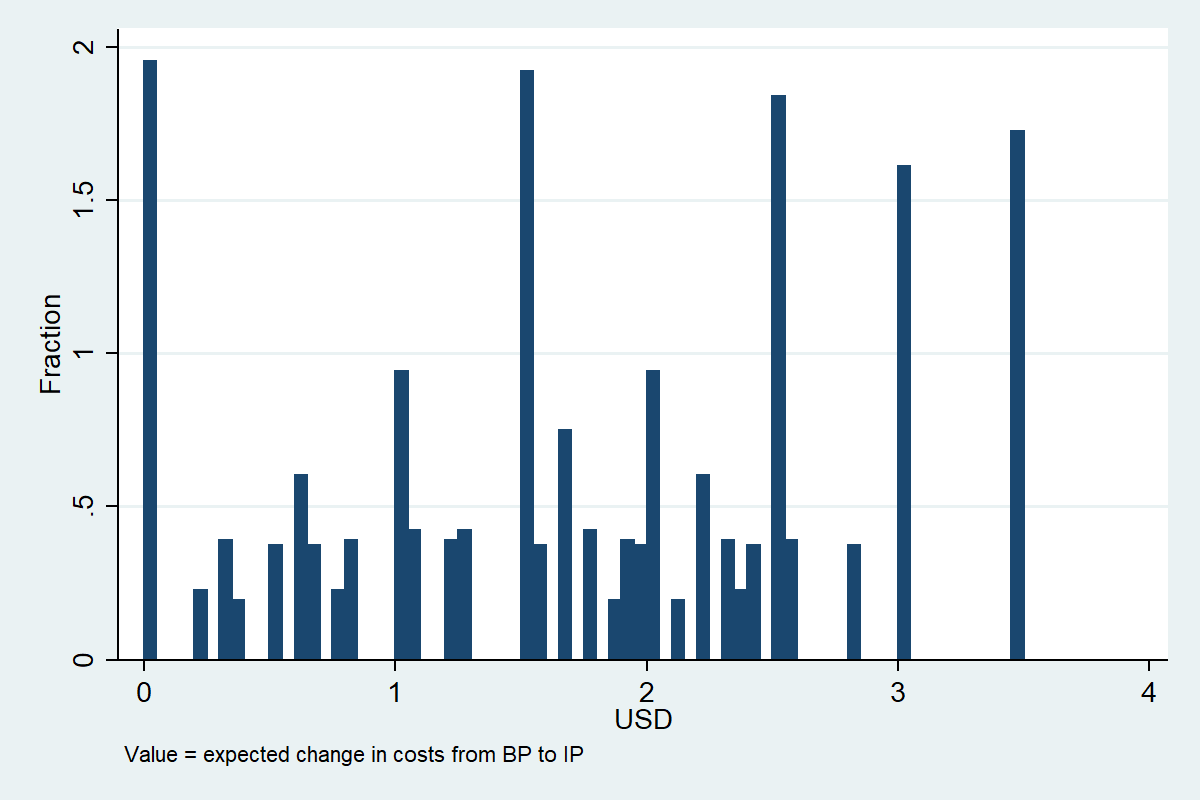
\includegraphics[width=0.8\textwidth]{Graphs/hist_value.png}
\end{figure}


\FloatBarrier

%\resumetocwriting
\newpage
\newpage
\section{Proofs}
\small

\subsection{Proposition 1}
%\small
\begin{proof} If protection costs are low enough $c<\pi L$ then a risk-neutral decision-maker should always protect without a signal:
$$U=\max[\pi(Y-L)+(1-\pi)Y,Y-c]=Y-c$$

It means that a strictly risk-averse decision-maker with a utility function $u()$ should also protect:
$$\pi u(Y-L)+(1-\pi)u(Y)<u(\pi(Y-L)+(1-\pi)Y)\leq u(Y-c)$$

Then denote stochastic payoff with a signal as $X$ so that expected utility with a signal is $Eu(X-b)$ where $b$ is the willingness-to-pay solving:
$$Eu(X-b)=u(Y-c)$$
 Let $b_0$ be the willingness-to-pay for a risk-neutral decision-maker. By (strict) Jensen's inequality:
$$Eu(X-b_0)<u(EX-b_0)=u(Y-c)=Eu(X-b)$$

Because $u(\dot)$ is an increasing function we obtain $b<b_0$. \end{proof} 

\subsection{Proposition 2}
%\small
\begin{proof}
Use the mean value theorem to rewrite the sensitivity as:
$${db\over dP_{01}}=-{\pi u'(\zeta)(L-c)\over E[MU]},\zeta \in \left(Y-L-b, Y-c-b\right)$$
Now let $X$ denote a (random) payoff of the agent with a signal. A risk-averse decision-maker puts a positive value on the signal only if its expected payoff is higher than the certain payoff with full protection: $EX>Y-c-b$. If an agent is imprudent ($u'''<0$) then $u'(\cdot)$ is a strictly concave function and hence $E[MU]\equiv E[u'(X)]<u'(EX)$ by Jensen inequality. Next, $u'$ being a strictly decreasing function due to strict risk aversion and $EX>Y-c-b$: $u'(\zeta)>u'(Y-c-b)>u'(EX)$. Hence ${u'(\zeta)\over E[MU]}>1$ and ${db\over dP_{01}}<-\pi(L-c)$. 
\end{proof}
%\normalsize

However, risk aversion can both increase and decrease subject's sensitivity to false-positive rates depending on the utility function curvature and signal's characteristics. Intuitively, an expected marginal utility of a strongly risk-averse subject with an imperfect signal can be lower than the average slope of the utility function between ($Y-c-b$) and ($Y-b$) which reduces sensitivity to false-positive rates. It can also be higher if either the signal is good or the curvature is small.


\subsection{Proposition 3}

\begin{proof}


Sensitivities to FP and FN rates are given as:

\begin{equation}
	{db\over dP_{10}}=-{(1-\pi)(u(Y-b)-u(Y-c-b))\over D(\pi, P_{01}, P_{10}, b)}
\end{equation}
\begin{equation}
	{db\over dP_{01}}=-{\pi(u(Y-c-b)-u(Y-L-b))\over D(\pi, P_{01}, P_{10}, b)}
\end{equation}


Hence the ratio of sensitivities is:
\begin{equation}
{db / dP_{01}  \over db / dP_{10}} = {\pi \over (1-\pi)} {(u(Y-c-b)-u(Y-L-b))\over (u(Y-b)-u(Y-c-b))}
\end{equation}


Based on the mean value theorem, there exist such $\zeta_1 \in (Y-L-b, Y-c-b)$, $\zeta_2\in (Y-c-b,Y-b)$ that $u(Y-c-b)-u(Y-L-b)=u'(\zeta_1)(L-c)$ and $u(Y-b)-u(Y-c-b)=u'(\zeta_2)c$. Hence we can write:

\begin{equation}
{db / dP_{01}  \over db / dP_{10}} = {\pi \over (1-\pi)} {u'(\zeta_1)(L-c)\over u'(\zeta_2)c}= {\pi (L-c)\over (1-\pi)L}{u'(\zeta_1)\over u'(\zeta_2)}
\end{equation}

Because $\zeta_1<Y-c-b<\zeta_2$ and $u''<0$, $u'(\zeta_2)<u'(\zeta_1)$ and hence:
\begin{equation}
{db / dP_{01}  \over db / dP_{10}} = {\pi \over (1-\pi)} {u'(\zeta_1)(L-c)\over u'(\zeta_2)c}>{\pi (L-c)\over (1-\pi)L}
\end{equation}
Because the last expression on the right describes a ratio of sensitivities for a risk-neutral agent, we obtain that strictly risk averse subjects exhibit higher relative sensitivity to FN rates. 

\end{proof}




\newpage
\section{Subjects' Explanations}
\footnotesize
The list of responses to the question \textit{''Please explain the strategy you used for Task 2 (Informed Protection)? This is the task in which you see a hint and when decide to protect or not.''}:
\begin{enumerate}
\itemsep0em 
\item if the hint was favorable not protection and vice versa
\item I always bought protection unless I was certain that I didn't need it (i.e. both gremlins were honest or it wasn't possible to get the black/white gremlin)
\item I trusted honest golems fully, and did not put much stock in the swamp golems.
\item my strategy was to just look at what the odds were
\item I looked at the percentages of white and black balls and made my guess off of that. Also, there was no big harm in buying protection, and there was a lot of harm if you did not buy protection and got a black ball.
\item I trusted my instinct.
\item If the entire panel of gremlins was honest and they told me that the selection was white, I did not buy protection, since I could be certain that I would not lose money. In any other scenario, I bought protection. In my case, better to guarantee a \$25 return every time than risk \$20 for a \$5 reward.
\item if it is an honest one, i don't need to buy informed protection cuz i can't trust its hint.
\item I think the gremlins were confusing, but if you see how many gremlins were. Then from that how many of each type where and what they say, after that you based that to the actual percentage of balls you get close to the answer.
\item I am a little bit more risky so I chose to not get protection if any of the monsters said it was white because I felt the probability of one of the honest ones getting picked was higher and if they said it was black I bough protection.
\item i used probablity and if the odds were more in favor i would mae a decision based on that and the ball probabilty color
\item If the hint was from one of the honest gremlins then I didn't choose to protect because they could only tell the truth. If there were any just black or just white gremlins then I decided to protect because the information they give isn't helpful

\item See the quantity of hints and the percentage of drawing the colors of the balls.

\item I would calculate the probability that the gremlins were right. So in task two, I already did task 3. Like if there were two black/white gremlins, I would add the probability that they were right to the certainly that the honest gremlin was right.

\item I would see what the probability that they are telling the truth is and then see if they were saying black. if no one was the black swamp monster then I knew it was black and therefore it would be 100\%

\item I looked at the box of balls and the box of gremlins. If the gremlins were honest or white, I would not use protection for a white ball. If the ball was black I would sometimes take my chances depending on the amount of white and black balls. If they were honest or black, I would use protection for a black ball. If the ball was white, I would not use protection since there were mostly honest gremlins.

\item I weighed the cost of loosing money and percentage difference with that chances of getting a white ball.

\item I weighed my odds. I knew they were in my favor.

\item When I paid attention to the composition of the box and saw the gremlins, that helped to inform my decision on whether to buy protection. For example, if I saw the box had equal numbers of both black and white ball and two honest gremlins were there, I did not buy protection. When I saw a box with a larger amount of black than white balls and had a white-swamp gremlin with four honest gremlins, I opted to buy protection.

\item I would the probability of one of the balls being picked. If the chances were not likely than I would not protect it.

\item I looked at what percentage of gremlins were honest and used that info in my decisions.

\item Instinct and possibility of either white or black being picked

\item I took protection when there was a higher chance of drawing out black balls.

\item If all glimpses are honest, then choose not to protect on each color. If most are honest and one is black, then choose not to protect white color. If the one is white, then choose not to protect black because we know white one always say white, so black color should be the truth.

\item I based my decision on the probability of the honest gremlin being chosen.

\item I would base my answers off of how many honest goblins there were.

\item I chose the best odds

\item If it was more than approximately a 70\% chance of drawing a black ball, I decided to protect. The cost to protect outweighed the potential loss of not protecting.

\item If the gremlin was honest then I did not buy protection because they were accurate in telling me the color of the ball.

\item If there were only honest gremlins then I never protected but even if there was one white-swamp gremlin or one black-swamp gremlin then I payed for protection.

\item If the gremlins were honest, I didn't buy protection. If there were swap gremlins, I calculated the chance of getting a hint from a swap gremlin and considered that along with the chance of getting a black ball. If the total chance of getting a black ball was more than 15\% I get protection.

\item I determined what the probability was that the gremlin would tell the truth. The more honest gremlins in the lineup, the less likely I was to buy protection. However, I'm risk-averse, so I was more likely to buy protection than not because the risk was too high and the cost of protection was low.

\item I just used probability in my head

\item \textbf{I took into consideration how many honest there were and looked at the chances of picking a ball}

\item I was able to calculate the odds from the hints. It was not a measurement requiring me to calculate the chance of balls, but of variance between the hints. This made it easier to calculate the probability of what the chances the gremlins would give regardless of the actual odds (14/6 white-black balls)

\item I just took into note the goblins that were listed, and then the probability of which the information could be truthful or not.

\item I just relied on the number of honest gremlins to inform my decisions

\item If there were a white swamped gremlin, I would buy the protection if it said white ball. If it said black on a white swamped I would always not buy the protection. This is vice versa if there was a black swamped gremlin.

\item I used the strategy of using the ``honest gremlin" to my advantage to know when I could get away with not paying for protection

\item I relied on understanding which type of gremlin was presented and then based my decision on their bias/lack of bias. Honest gremlin were a simple binary decision (white -> no protection, black -> protection). The white gremlin would default to no protection unless the probability of black was greater than 25\%. The black gremlin defaulted to protection.

\item I considered the probability of the computer selecting a white ball and a honest gremlin. If that probability was high ($>$70\%), then I decided not to buy protection. When there were only honest and black gremlins and the hint was that the ball was white, then it was easier since that hint could only come from an honest gremlin.

\item I took into consideration which of the gremlins I got. If it were two honest ones, I would not buy protection if they said white because they were right. If they were two honest ones and a black one, and they said it was white, I would do the same thing because the black one would never say the ball is white. If any of the gremlins said the ball was black, I would buy protection because there would always be a chance that the ball was black.

\item It was really just similar to math and common sense.

\item I went with the odds. I didn't buy protection if the probability of picking a ball was really high in a situation

\item I would look at how many honest gremlins there were to see if i could trust it or not. ex: if there were only honest and white gremlins, and they said the ball was white, i would trust that.

\item If it was all honest then I 100\% percent trusted it and went for no protection but if there was even a chance of dishonest gremlin then I went with protection

\item My strategy depended on the gremlins. I was willing to pay a higher price for more honest gremlins, while I was not willing to pay as much when there were not as many honest gremlins.

\item The higher the \% of black balls the more likely I was to buy protection.

\item I based it off of the amount of different colored balls mainly. Because, if there was only 2 black balls and one black gremlin, then I would most likely have a white ball chose if the other two were honest.

\item I looked at the percentage and the chance of drawing which ball, and I compared it to the grimlin options/hints and made my decision based off of the numbers I was provided.

\item I am broke and I was willing to take risks to make more money.

\item I just hoped for the best and picked one

\item \textbf{If it was all honest gremlins I did not buy protection. Even if there was one un honest gremlin I was skeptical to buy protection. If there was more than one un honest gremlin I definitely bought protection.}

\item If there were more black balls I would decide to protect it because there was a higher chance it needed to be and if there were more white balls I didn't protect it because I assumed the chance of a black ball being chosen was lower.

\item My strategy in task two was primarily based on the gremlins. For example, if they were all honest then I would not buy protection if they said white but would if they said black. Furthermore, if four were honest and one was a white-choosing gremlin, then if the gremlins said the ball was black I would buy protection; Considering that the white gremlin could only say the ball would be white, then it is known that an honest gremlin said that the ball would be black and vise versa. I did not really consider the probability of the balls being chosen and rather focused on the likely hood that the hint given by the gremlins is correct.

\item I would first take into account how many white and how many black balls were in a box, and the chance of drawing each. With the gremlins then telling a hint I would not buy protection if the gremlin said white and the percent of drawing white was more than 75\%. I used this kind of method for the whole task.

\item my strategy for this task was to only buy protection if there was a white or black gremlin and not if there was a truth gremlin

\item the percentages of black and white balls and which gremlins I would get to give a hint.

\item I took my chances that the gremlins telling the truth would be selected

\item If the goblins were all honest I would buy protection if they say the black was the ball chosen and not if the ball was white. If 1 of the goblins was saying the ball was black or white exclusively I would buy protection if they say it was black and not if the ball was white. If 2 of the goblins was saying the ball was black or white exclusively I would buy protection no matter what they said

\item How likely it was that it would be white

\item I mainly looked at the probability percentage of the computer choosing a white ball. If it was greater than or equal to 70\%, then I would not choose protection.

\item It was pretty simple, actually. I basically based my decision off of the amount of honest gremlins there were. If there were 4/5 honest, then there was an 80\% chance the hint was correct. On a situation with 50\% white and 50\% black, this strategy proved to be helpful.

\item I based my decision off of the makeup of the gremlins if they were all honest and said the ball was white I would not buy protection and if they said it was black I would buy protection. If there was a 1/3 chance of an honest gremlin being picked for the hint I would just buy protection because I did not like the odds of the hint being true. If the chance of an honest gremlin being picked was 2/3 I would look at the probability of a white/black ball being chosen and then make my decision to protect or not off of that.

\item I based my chances solely on the honest Gremlins.

\item I mostly would buy protection if there was an over 50 percent chance to get a black ball.

\item I thought of how many un honest gremlins there were and tried to guess the percent of accuracy I would be given based on the colors.

\item If it was mostly Honest Grimlins I took the hint

\item I looked at the different types of gremlins in each group to make my decision. If it was all of the honest gremlins, I would go from there, but even if it were 2 honest and 1 black or white swamp gremlin that would inform my decision better than if it was an equal mix of all three types

\item I looked at the \% of white vs black balls then looked at how many honest grimlins there were. If there were a majority of white balls and honest grimlins I would do no protection for a white ball but buy protection for black.

\item Always went with the honest ones. When there was one white or one black, I would know it was an honest one when they said the opposite of the color. For example, two honest and one white, when it said the ball was black, I knew it would be black because the white can't say that.

\item I compared the number of balls to the gremlins hints and if the chances were higher than 50\% ish I wouldn't get protection

\item I would always take the hints from honest and be skeptical of non-honest

\item I looked at the gremlins and then looked at their hint. depending on what gremlins I had, i looked at the combination of balls to see if I should risk it or not. If I had a lot of white balls and quite a few honest gremlins, I did not buy the protection plan

\item I decided weather or not to buy protection based on the gremlins

\item I am basically gambling so I would not pay attention to the Gremlins and look at the percentages

\item Sorry. My strategy was same through-out, except the very first question of task1. Risk-averse, not worried about losing \$5. Also, not trusting even honest gremlins or perhaps myself if I had mis-read.

\item Just went with my gut guess. I didn't really use a strategy for any of them tbh

\item there was no need to protect if the hint were made by all honest gremlins. also no need to protect if i had a combination of honest and black gremlin and the prediciton said it's white cos a black gremlin will never give a white answer

\item I had two honest gremlins, so the hint was 100\% accurate.

\item I measured my decision based off of the type of gremlin giving the hint. If I felt that the gremlin or group was highly trustworthy, I would follow the advice.

\item If it was highly likely that the gremlin was going to be correct, I chose no protection. I aimed for the highest payout each round based on the amount of black to white balls there were.

\item If there were all honest ones I would not buy protection if it was white. I bought protection on all the others so that I would not lose more money.

\item I just created a pattern in my head and looked at the percentage of the likeliness of a black ball being drawn or not.

\item I based it off the amount of honest gremlins presented

\item If the color said was the opposite of black or white eyed gremlin then I knew it was true because the rest were honest gremlins

\item Based off how many white ball there was

\item I decided what to do based on both probability of selecting a ball of off composition of colors, and the used the gremlins to add an extra level of certainty.

\item Simply used the projection of likelihood for how much risk I was willing to take.

\item If i was feeling lucky or not

\item Based off of the number of gremlins would help me determine to use protection or not

\item I used the gremlins as my strategy, i took more risks if it was the honest gremlins

\item I payed attention to the honest gremlins and I used my answers based off how many there were.

\item I would observe which of the gremlins informing me were honest and make my decision there.

\item I just tried not to risk it. I prefer getting a little bit less than the total amount than actually reducing \$20

\item I figured out what the gremlins were saying and used that to calculate the probability

\item I just guessed.

\item I thought about which option would make me the most amount of money based on protection or not.

\item I just decided which ones wanted protection and not.

\item Basically if the white balls had a higher rate than the black balls I wouldn't buy protection

\item I looked mostly to whether or not I had an honest gremlin in my group. If I had gremlins which could be dishonest, I then evaluated my chances based on the percentage of black vs. white balls in the box.

\item If I knew the ball would be white then I would not protect, everything else I protected

\item I was a little more clueless about it, I tried to make sense of the question first and then see the number of balls that were black and if they were less, then I would not buy protection.

\item If the goblins were guaranteed to be honest, I followed their hint. If there was a white goblin at all, I ignored the hint completely. If there was only a black goblin, I wouldn't buy protection if the hint was white since that couldn't be correct.

\item I took a chance each time
\item If there was all honest gremlins, I would not protect unless they said the ball is black. If there were white or black gremlins in the mix, I generally chose to protect unless the chances the ball was white were greater than 90\%.
\item If there was ever a question I always bought protection because I would rather have 25 dollars than 10.
\item It really depended on how many balls were in the box 
\item anything under 80\%. I know what my time is worth and don't want to waste it for \$5 unless my return was greater then the odds I would be given. 
\item I would try to think back to what the amount were if i choose protected v.s unprotected. 
\item I would calculate the possibility in my head each task.
\item I decided whether to trust my informed protected based on how many gremlins were present divided by how many gremlins were honest/would say if the ball was white or black. I was more likely to trust the honest gremlins or buy protection for the dishonest gremlins.
\item If I new the odds of the hint gremlin is honest then I would protect baes on the hint they made
\item if it was mainly honest ones and the probability was an 80/20 split i just took my chances 
\item Seeing the probabilities and protentional outcomes were what played a role in decision making.
\item if it is white never by protection, if it is black always buy protection. There is a higher chance that 1 a ball is white, and 2 that the gremlin is honest so it makes sense 
\item examine the beasts, then make a decision
\item if all the gremlins were honest and said white i would not protect. If all the gremlins were honest and said black i would protect. If the gremlins were honest, honest, black and the hint was white, i knew it was one of the honest gremlins that was giving me the correct answer of white, so i didnt protect.
\item Odds based on the original sample times the odds of the gremlins giving bad info
\item I just thought there would no way the black ball would be chosen if there was only 1 or 2 of them. I was just trusting my guts. 
\item mainly it was for the 70/30 i reled on the hits if it was black to think what are the changes it is realy black and if do then buy the protection. often it was more favored of the white being true to dont need the protection
\item If all the Grimmlies where honest I did not use protection, if they weren't I used protection. 
\item I first looked at the chance and if it was 90\% white 10\% black, I probably didn't buy protection or 50 cents at most. Then, I looked at the gremlin and if they were only honest ones I was willing to pay up to $2. If there were white/black gremlins and there was a high chance of black balls I figured I would pay up to $1 just incase. 
\item GAMBLING
\item So the strategy that I used are to look at the box and see how many honest gremlin there were and decide if I wanted to protect or not. 
\item I didn't realize it told me my odds of the balls at the top of the screen so i went based off of the gremlins i had again. I got a lot of honest gremlins so anytime i had a white or black one because i never had both in on grouping it was normally 2 honest or like 4 honest and 1 black or white gremlin so then i would go off of the answer that was opposite of what the white or black gremlin was cause how could it tell me if the answer was a color it couldn't see.
\item I just guessed based on probability. 
\item every time it was all honest gremlins I never used protection, but after that I based my answers off the percentage of the white ball being drawn.
\item not needed unless over 50\%
\item always buy protection for guranteed money
\item if they were honest gremlins i said what they said, if there was a smaller amount of gremlins i would pay for protection but iuf there was a larger amount of gremlins i would put both as not paying for protectin
\item I would measure the chances that the hint would be useful in addition to the actual percentage that the ball would be a certain color
\item If I had majority of honest gremlins, I would most likely follow the hint. The more swamp gremlins I had the less I would follow the hint.
\item High risk, high reward 
\item If the odds were favorable to me without the hint i wouldnt take it. If i got bad gremlin luck i would not take hint. If the honest gremlin said white and the white gremlin was there I would take the hint
\item If they were honest gremblins then I trusted that whatever they said was correct, but if there was one of each I added protection because it then wasn't as sure, especially if it was 90\% to 10\%. 
\item If the gremlins were honest, then I would take the hint. If they were not, then I did not want to take that chance.
\item If they are all truth then you don't have to worry. If they are all truth and then 1 black but it says white, you dont have to worry. After that i did mental math to see what was the likelihood one of the liers get drawn and then what percentage of the remaining data would be effected. 
\item Well for a white ball there's really no penalty to protect it so you would be wasting money to protect it. For a black ball it depends, because if there's a black eyed gremlin paired with a honest gremlin then take you chances with the protection, but if there's a white eyed one paired with a honest gremlin then its false because that would never happen. 
\item I just used math and assigned a value to how much the hints provided help and went from there
\item Counting the ratio of white to black dots
\item I always took the hint from honest gremlins or white only gremlins
\item I would always choose protection because the risk was too high if i did not choose it. But, if i had to honest gremlins i knew what they said was correct so i would not protect.
\item I pretty much just kept a basis of what I was willing to lose. If you purchase the informed protection but at too high of a cost, you lose out on key dollars over time. 
\item If it was 5 honest gremlins + 2 white gremlins and they were saying it was black, I would protect because the only option would be for the honest gremlins to be saying the truth about the ball.  If it was 5 honest gremlins and 2 black gremlins and they claimed the ball was black, I would have less of a certainty getting protection, and would see the actual proportion of the balls. 
\item I decided to not take the risk for most parts because 25 is a lot better than 10, even if it means you're losing \$5
\item I mostly used my chances of the balls (10\% black 90\% white) to make my decision and would only accept the hint if it dipped below 90\% and have that influence me.
\item I looked at the balls in the drawing pit and used those odds to determine my decisions.
\item All or nothing
\item I used deductive reasoning
\item Well I knew if it was all honest gremlins they were always correct, if it was all honest and like 1 or 2 black gremlins and i knew if the gremlin said white it had to be white and vice versa because that means the honest gremlin said the color as the other gremlins cannot say each others opposite colors. 
\item I decided to look at the number of white vs black balls to make my main decision.
\item Kinda looking at the eye balls because if it says white then the black gremling cant say that
\item if they were both honest, i did not protect if they said white because it was white and i did protect if they said black so that i would only lose $5 opposed to $20. with the white and black eyed, i then weighed my likelihood and decided based on the percentage of pulling and the percentage of them telling the truth
\item If 2 of the three swamp gremlins were honest, and the other was white, i knew that if a random 1 said white, my chances were 66 percent, but if they said black, my chances were 100 percent
\item I took into account the probability that I got an honest hint and then also the probability of the ball being black. If there was a 90\% chance of the ball being white, it was a waste of money to buy a hint regardless of the probability of it being honest or not.
\item The hints don't matter, the question was asking about \% likelihood and those numbers were provided.
\item I saw the gremlins and figured out what they would tell me, the truth, only white, or only black. I decided mostly based on the percentage of the ball actually being black. Because if the ball is most likely going to be white I won't need protection.
\item I mostly paid attention to how many black and white swamp monster things there were compared to the honest ones. If there was only one possible liar in the line up then the chances of not choosing correctly felt lower. 
\item Played it very risky and it paid off
\item I almost always decided to buy protection because it only cost \$5. 
\item I used statistics to calculate whether it was worth it or not. 
\item I used the given probability to decide if a paycut was statistically worth it
\item based on the chances of drawing a black ball and the hint recieved i made my decision
\item Using both the chances of the ball being white and what monsters I had 
\item If there were enough truths, i would bet more on it being truthful
\item I would assume that based off of probability i would get a truthfully dude, the odds were always 5:1 of them not lying so you play the odds
\item more white balls then black
\item This one was interesting
\item i usually chose to protect if there was 70\% chance or less
\item I looked at how many honest ones and non honest ones were accounted for.
\item I used percentage of balls in given box.
\item If there were more truth grimlins i tended to trust my decision more
\item If both gremlins were truth gremlins I listened, but if one was lying I bought protection for both.
\item If there were two honest gremlins then I would protect when given a hint that it was a black ball. With the others there was a 5/7 chance that I would get an honest gremlin, I should have protected when it said "black ball" in the case with 2 white gremlins. If there was a white and black gremlin I tried to base it off of the probability of actually drawing a white ball. 
\item I looked to see which gremlin was diplayed to determine my answers. If there were more honest gremlins then I would protect or not confidently. But if there were more dishonest gremlines then I would protect or not with doubt.
\item I looked at the probability of the balls colors as well as the types of things giving the hints. I would protect if there was a high chance of the ball being a certain color and if the hint could be false. 
\item I was just looking at what the odds of the black and white balls where and then which kind of gremlins I had then made my decision off that.
\item i decided to use a back and forth decision by buying and not buying protection
\item I kind of just used my best judgement and guessed a little bit.
\item If the Gremlins were both good hint ones I would not protect. If there was a good hint one and a white one I would protect on the white ball and the black, since the white gremlin can't say black, it would have to be the hint one. I did the same thing but opposite for the black and hint gremlins. 
\item I didn't have much of a strategy honestly I just looked at the goblins and guessed. 
\item My strategy for informed protection was fairly simple. I would take the hint because in my opinion 25 dollars is better than 10, or the risk of winning 30. I am a bit of a gambling man, but when the white and black eyed gremlins could have been lying about something they said I figured better to take the confirmed money than risk it for more. 
\item I did not get protection if it was likely that I would get a white ball.
\item Hints that are given from two truthful monsters are valuable so no protection is needed, because I know what they are telling be is the truth (if the ball is white). In all other cases I bought protection no matter what because I didn't want to risk losing a free \$25 by simply not buying protection.
\item If the gremlins were honest, I never protected, but if there were black or white-eyed gremlins at all, I would protect.
\item I played it safe and bought protection unless I liked the odds of getting a white dot or if I had two truth gremlins.
\item i just went off of the gremlins for each round
\item Just used what are the odds and logical thinking.
\item I looked at the probabilities, then made my decision based on the gremlins presented.
\item If I saw the trust swamp monster I didn't pay for protection.


\end{enumerate}

\newpage
\section{Experiment Instructions (for online appendix)}


%\captionsetup[figure]{list=yes}
%\captionsetup[table]{list=yes}

\renewcommand{\contentsname}{\vspace{-1em}}
%\tableofcontents

%\newpage\clearpage
\setcounter{table}{0}
\setcounter{figure}{0}
\setcounter{equation}{0}
\setcounter{footnote}{0}
\setcounter{section}{0}
\renewcommand\thesection{\Alph{section}}
\renewcommand\theequation{\thesection.\arabic{equation}}
\renewcommand\thetable{\thesection.\arabic{table}}
\renewcommand\thefigure{\thesection.\arabic{figure}}
\renewcommand\thesubsection{\Roman{subsection}}

\end{appendices}


\end{document}